\documentclass[times, utf8, diplomski]{fer}
\usepackage{booktabs}
\usepackage{listings}
\usepackage{xcolor}

\definecolor{verylightgray}{rgb}{.97,.97,.97}
\lstdefinelanguage{Solidity}{
	keywords=[1]{anonymous, assembly, assert, balance, break, call, callcode, case, catch, class, constant, continue, constructor, contract, debugger, default, delegatecall, delete, do, else, emit, event, experimental, export, external, false, finally, for, function, gas, if, implements, import, in, indexed, instanceof, interface, internal, is, length, library, log0, log1, log2, log3, log4, memory, modifier, new, payable, pragma, private, protected, public, pure, push, require, return, returns, revert, selfdestruct, send, solidity, storage, struct, suicide, super, switch, then, this, throw, transfer, true, try, typeof, using, value, view, while, with, addmod, ecrecover, keccak256, mulmod, ripemd160, sha256, sha3}, % generic keywords including crypto operations
	keywordstyle=[1]\color{blue}\bfseries,
	keywords=[2]{address, bool, byte, bytes, bytes1, bytes2, bytes3, bytes4, bytes5, bytes6, bytes7, bytes8, bytes9, bytes10, bytes11, bytes12, bytes13, bytes14, bytes15, bytes16, bytes17, bytes18, bytes19, bytes20, bytes21, bytes22, bytes23, bytes24, bytes25, bytes26, bytes27, bytes28, bytes29, bytes30, bytes31, bytes32, enum, int, int8, int16, int24, int32, int40, int48, int56, int64, int72, int80, int88, int96, int104, int112, int120, int128, int136, int144, int152, int160, int168, int176, int184, int192, int200, int208, int216, int224, int232, int240, int248, int256, mapping, string, uint, uint8, uint16, uint24, uint32, uint40, uint48, uint56, uint64, uint72, uint80, uint88, uint96, uint104, uint112, uint120, uint128, uint136, uint144, uint152, uint160, uint168, uint176, uint184, uint192, uint200, uint208, uint216, uint224, uint232, uint240, uint248, uint256, var, void, ether, finney, szabo, wei, days, hours, minutes, seconds, weeks, years},	% types; money and time units
	keywordstyle=[2]\color{teal}\bfseries,
	keywords=[3]{block, blockhash, coinbase, difficulty, gaslimit, number, timestamp, msg, data, gas, sender, sig, value, now, tx, gasprice, origin},	% environment variables
	keywordstyle=[3]\color{violet}\bfseries,
	identifierstyle=\color{black},
	sensitive=false,
	comment=[l]{//},
	morecomment=[s]{/*}{*/},
	commentstyle=\color{gray}\ttfamily,
	stringstyle=\color{red}\ttfamily,
	morestring=[b]',
	morestring=[b]"
}

\lstset{
	language=Solidity,
	backgroundcolor=\color{verylightgray},
	extendedchars=true,
	basicstyle=\footnotesize\ttfamily,
	showstringspaces=false,
	showspaces=false,
	numbers=left,
	numberstyle=\footnotesize,
	numbersep=9pt,
	tabsize=2,
	breaklines=true,
	showtabs=false,
	captionpos=b
}
\begin{document}

% TODO: Navedite broj rada.
\thesisnumber{2546}

% TODO: Navedite naslov rada.
\title{Ulančani blokovi i raspodijeljene glavne knjige s ograničenim pravom pristupa i pametnim ugovorima}

% TODO: Navedite vaše ime i prezime.
\author{Martin Pavić}

\maketitle

% Ispis stranice s napomenom o umetanju izvornika rada. Uklonite naredbu \izvornik ako želite izbaciti tu stranicu.
\izvornik

% Dodavanje zahvale ili prazne stranice. Ako ne želite dodati zahvalu, naredbu ostavite radi prazne stranice.
\zahvala{}

\tableofcontents
\listoffigures

\chapter{Uvod}
Baze podataka su posvuda.  Koristimo ih svaki dan. Na primjer, popis kontakata u mobitelu je jednostavna baza podataka - elektronička verzija papirnatog adresara. Detaljnije baze podataka uključuju popise kupaca, zaposlenika, pacijenata ili glasača i njihove svojstva i odnose. Složenije baze podataka mogu sadržavati čak i programe koji mogu međusobno komunicirati. Zapravo, o bazi podataka možemo razmišljati kao o bilo kojem organiziranom skupu informacija koje možete pro- naći i eventualno ažurirati stavke. Otkako je računalna revolucija započela pedesetih godina prošlog stoljeća, baze podataka igrale su važnu ulogu u poslu i društvu.

Mnoge su baze podataka danas dijeljene. Do sada je svijet toliko povezan da različiti ljudi često trebaju pristupiti istim podacima. Da bi se udovoljilo ovoj potrebi, pojavile su se distribuirane baze podataka, u kojima određenim dijelovima podataka može pristupiti više osoba odjednom. Primjerice, radi pojednostavljenja postavlja- nja ili ponovnog zakazivanja sastanaka, svi članovi radne skupine mogu dijeliti svoje sastanke na internetskom kalendaru. To se ne može učiniti s papirnatim kalendarom. Naravno, u poslu se koriste složenije zajedničke baze podataka. Neka od pitanja koja možemo postaviti pri radu s bazama podataka.

\begin{itemize}

\item Vjerujete li onome s kime dijelite podatke?

\item Kako možete znati da je netko onaj za koga kaže da je?

\item Što smiju raditi s bazom podataka?

\item Tko rješava sukobe ili sporove?

\end{itemize}

Jasno je da postoji mnogo praktičnih problema s dijeljenjem baze podataka. Tijekom vremena ljudi su isprobali mnogo različitih rješenja. Jedan uzbudljiv novi način dijeljenja baza podataka koji može pomoći u rješavanju tih problema je tehnologija ulančanih blokova (eng. Blockchain). 

\begin{figure}[htb]
\centering
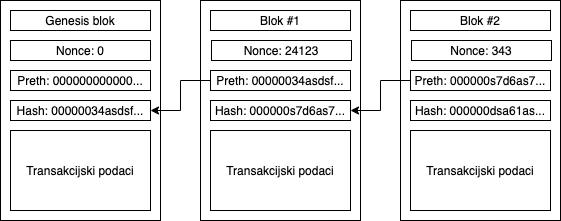
\includegraphics[width=12cm]{imgs/Blockchain.png}
\caption{\textit{Blockchain}}
\label{fig:blockchain}
\end{figure}

Blockchain je tehnologija koja stoji iza Bitcoina. Mediji su prepuni priča o Bitcoinu i drugim kriptovalutama. Većina tvrtki ne brinu previše o kriptovalutama. Većina tvrtki je sretna što kupuje i prodaje s dolarima, eurima, funtama,  jenima ili bilo kojom drugom prihvaćenom valutom - možda čak i kriptovalutom - sve dok to djeluje za njih. Za poduzeća je daleko značajnija tehnologija koja stoji iza kriptovaluta, tzv \textit{\textit{blockchain}}.

Blockchain je novi oblik zajedničke baze podataka.  Blockchain je distribuirana baza podataka bez središnjeg tijela i bez točke povjerenja. Kada želite dijeliti bazu podataka, ali nemate puno povjerenja u druge ljude koji bi mogli koristiti tu bazu podataka, blockchain vam može biti od velike pomoći. U tom kontekstu, "povjerenje" može značiti mnogo stvari. Povjerenje bi moglo značiti vjerovanje drugima da će s bazom podataka postupati ispravno. Povjerenje bi moglo značiti da jedna strana drugoj ne pokušava doći do privatnih informacija. Ili povjerenje može značiti ne ponižavanje tuđeg učinka radi stjecanja konkurentske prednosti.

Rasprava o povjerenju otvara dvije glavne vrste blockchaina. Većina kriptovaluta koristi blockchain bez dozvola gdje se svatko može pridružiti i imati puno prava na njegovo korištenje. Na primjer, svatko može kupiti Bitcoin ili Ether jer oni koriste širom otvorene, blockchaine bez ograničenja pristupa. S druge strane, poslovni blockchaini imaju tendenciju da im se ne može pristupiti bez dozvole. To znači da osoba treba ispuniti određene zahtjeve za izvođenje određenih radnji na blockchainu. Neki blockchaini ograničavaju pristup čak i prethodno provjerenim korisnicima koji su već dokazali da su oni za koje kažu da jesu, što se može dogoditi kada postoje podatci na blockchainu kojima mogu pristupiti samo određeni sudionici. Drugi dopuštaju bilo kome da se pridruži, ali dopuštaju samo provjernim identitetima da verificiraju transakcije na blockchainu.

U bazi podataka koju dijele dvije različite stranke postavlja se pitanje, što se događa ako obe stranke žele pristupiti podatcima u isto vrijeme? Ako bi se tom bazom podataka upravljalo s blockchainom, ovaj bi se problem mogao riješiti kroz proces koji se naziva konsenzus. Blockchaini koriste konsenzusne sustave kako bi bili sigurni da su podaci u bazi podataka uvijek ispravni. Primjerice, konsenzusni sustav koristio bi unaprijed utvrđena pravila za određivanje koja stranka prva dobiva pristup podatcima. Konsenzusni sustavi imaju mnogo različitih oblika s različitim imenima. Na primjer, Bitcoin koristi dokaz izvršenog rada (eng. proof of work, skr. PoW) konsenzus, gdje računala sudionika rješavaju teške matematičke zadatke. Najbitnije svojstvo koje takvi sustavi moraju zadovoljavati naziva se \textit{Byzantine Fault Tolerance} ili skraćeno BFT. 

Zašto je blockchain važan poslovnim ljudima? Pomoću blockchaina mogu se usmjeriti mnogi postojeći poslovni procesi u mnogim industrijama kako bi uštedjeli vrijeme, uštedjeli novac i smanjili rizik. Mnogi potpuno novi procesi - možda čak i potpuno nove industrije mogu biti izumljeni. Prva generacija interneta bila je izvrsna za dijeljenje informacija: stvari poput e-pošte, dokumenata, fotografija, web stranica, pjesama i videozapisa, ali postojao je problem. Bilo je teško nekome dokazati da su oni koji su rekli da jesu. Svaka transakcija koja je uključčivala bilo koju vrijednost zahtijevala je posrednika, poput banke, da potvrdi kupca i prodavača i potvrdi transakciju. To je stvorilo trenje, kašnjenje i trošak - i središnja točka neuspjeha koju bi napadači mogli napasti. Blockchain otvara vrata drugoj generaciji interneta za koju je mnogo prikladnija razmjena vrijednosti, uključčujući vrijedne informacije. Pomoću blockchaina ljudi mogu utvrditi tko su i zatim mijenjati stavke poput novca, dionica i obveznica, intelektualno vlasništvo, djela, glasove, bodove lojalnosti i sve ostalo što ima vrijednost. Čak i ako se stranke ne znaju ili ne vjeruju jedni drugima, mogu vjerovati tehnologiji za bilježenje transakcija. A tehnologija uklanja potrebu za bilo kojim posrednikom, što štedi vrijeme i smanjuje troškove.

\chapter{Blockchain s ograničenim pravom pristupa}
Postoje razne arhitekture blockchaina. S ograničenjem pristupa i bez ograničanja pristupa, javni i privatni. Nama su, u ovom radu, najzanimljivija arhitektura blockchaina koja ima ograničen pristup. Takvi blockchaini zahtijevaju posebna dopuštenja za čitanje, pristup i upisivanje podataka na njih. Suštinska konfiguracija takvih blockchaina kontrolira transakcije sudionika i definira njihove uloge u kojima svaki sudionik može pristupiti i doprinijeti blockchainu. To također uključuje i održavanje identiteta svakog sudionika blockchaina na mreži. Takvi se blockchaini nazivaju blockchaini s ograničenim pravom pristupa (eng. permissioned blockchains, skr. PBs). PB-i također se razlikuju od privatnih blockchaina, koji omogućuju sudjelovanje samo poznatim čvorovima. Na primjer, banka možda pokreće privatni blockchain koji posluje kroz određeni broj čvorova unutar banke. Suprotno tome, PB-i mogu dopustiti bilo kome da se pridruži mreži nakon što se definiraju njihov identitet i uloga.

\textbf{Prednosti}. Brojne su prednosti blockchaina s ograničenim pravom pristupa, koje ga čine povoljnijim za upotrebu od javnih blockchaina. PB-e karakterizira učinkovitija izvedba. Kada bi uspoređivali PB-e i javne blockchaine, oni nude bolju izvedbu. Glavni i najočigledniji razlog tome je ograničen broj ččvorova koji sudjeluje u blockchainu, za razliku od javnih blockchaina gdje, u teoriji, može biti neograničeni broj ččvorova. Iz toga slijedi uklanjanje nepotrebnih proračuna potrebnih za postizanje konsenzusa, što svakako poboljšava izvedbu i performanse, a još i k tome imaju unaprijed određene čvorove koji validiraju transakcije. PB-i imaju pravilno organiziranu strukturu upravljanja, što rezultira tome da administratori trebaju manje vremena za ažuriranje pravila mreže, što je značajno brže u odnosu na javne blockchaine. Jedan od problema javnih blockchaina je taj što ne rade svi čvorovi zajedno kako bi implementirali ažuriranja mreže. Čvorovi mogu staviti svoje vlastite interese iznad interesa cijelog sustava, što rezultira usporavanjem ažuriranja mreže. Za usporedbu, PB-i nemaju taj problem jer čvorovi unutar takvog sustava rade zajedno kako bi brže ažurirali mrežu, i zato što si međusobno vjeruju i surađuju, u interesu im je da je mreža što bolja i funkcionalnija. Jedna od vrlo važnih karakteristika koja pridonosi korisnosti PB-a je decentralizirana pohrana. PB-i potpuno iskorištavaju tehnologiju, tako što osim samih transakcija koje se događaju na mreži, također spremaju i druge važne podatke koje svi (ili neki) ččvorovi u mreži koriste. Ti su podatci spremljeni između čvorova organizacija koje su sudionici PB-a, a održavaju se jednakima za sve konsezusnim algoritmima. Sve to dovodi do toga da PB-i zahtijevaju manje troškova od drugih modela poslovanja te možemo zaključiti da su isplativi, pogotovo u usporedbi s javnim blockchainima, gledajući iz perspektive poslovnih rješenja.

\textbf{Nedostaci}. Naravno, PB-i nisu oslobođeni nedostataka. Sigurnost PB-a dobra je koliko i integritet člana. Maliciozni dio PB-a može promjeniti i ugroziti podatake pohranjene u mreži. Na taj se način može ugroziti integritet mreže. Da bi ga riješio, sustav treba imati odgovarajuća dopuštenja, tako da se loši čvorovi ne mogu udružiti i kompromitirati mrežu. Kontrola, cenzura i regulacija - u idealnom svijetu PB-i bi trebali funkcionirati kao javni blockchain, ali s propisima. Međutim, propisi uvode cenzuru u mrežu, gdje tijelo može ograničiti transakciju ili kontrolirati da se ona dogodi. To je prijetnja bilo kojoj tvrtki ili organizaciji koja koristi PB. Ovaj pristup također onemogućuje PB da maksimalno iskoristi cijeli blockchain ekosustav.

\section{Konsenzus}
Svi čvorovi koji sudjeluju u mreži moraju se složiti oko svake poruke koja se prenosi između čvorova. Ako je grupa čvorova oštećena ili je poruka koju oni prenose oštećena, ona ipak ne bi trebala utjecati na mrežu kao cjelinu i trebala bi se oduprijeti ovom "napadu". Ukratko, mreža se u cijelosti mora složiti oko svake poruke prenesene u mreži. Ovaj se sporazum naziva konsenzusom. Konsenzus je temeljni problem distribuiranih sustava otpornih na kvarove. Konsenzus pokušava riješiti problem Bizantskih generala
(eng.  \textit{Byzantine Generals Problem}). Analogija korištena za problem Bizantskih generala u osnovi ide ovako: Nekoliko divizija bizantske vojske smješteno je neposredno ispred neprijateljskog grada i priprema se za bitku. Razni generali mogu međusobno komunicirati samo putem glasnika. Moraju se dogovoriti oko zajednikog djelovanja. Međutim, moramo pretpostaviti da su neki generali izdajice koji žele spriječiti lojalne generale da se dogovore oko zajednikog postupka. Potreban je algoritam kako bi se osiguralo da mala skupina izdajica ne može poremetiti komunikaciju. Da bi riješili problem bizantskih generala, lojalni generali trebaju siguran način da se dogovore o planu - konsenzus - i izvrše svoj odabrani plan.

\subsection{Dokaz izvršenog rada i dokaz uloga}
Dokaz izvršenog rada i dokaz uloga su dva najpoznatija konsenzusna algoritma koja se koriste unutar javnih blockchain sustava. Iako se u ovom radu nećemo baviti njima, važno ih je spomenuti jer su oni, posebno PoW, glavni čimbenici koji su pridonijeli razvoju današnjih blockchain sustava.

\begin{figure}[htb]
\centering
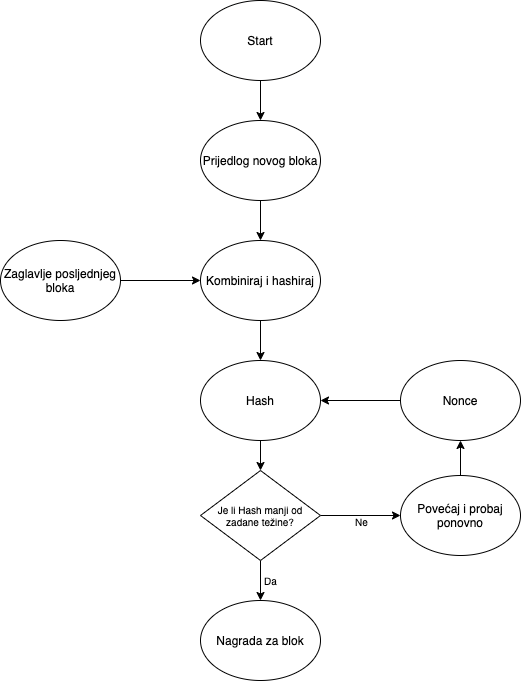
\includegraphics[width=12cm]{imgs/PoW.png}
\caption{Dokaz izvršenog rada}
\label{fig:pow}
\end{figure}

Dokaz izvršenog rada radi tako da rudari pokušavaju generirati hash koji je manji od zadanog praga koji se zove težina rudarenja. Do toga hasha dolaze tako da mjenjaju ulaz u kriptografsku hash funkciju dodavajući jedan cijeli broj koji se zove \textit{nonce}.  Dokaz izvršenog rada funkcionira na način da je vjerojatnost rudarenja bloka proporcionalna količini računalnih resursa rudara. Isplate za blokove vremenom postaju sve manje, kako bi se smanjila mogućnost većinskog napada na mrežu. PoW sustavi vremenom postaju centralizirani, jer se rudari udružuju u takozvane "bazene rudara".

\begin{figure}[htb]
\centering
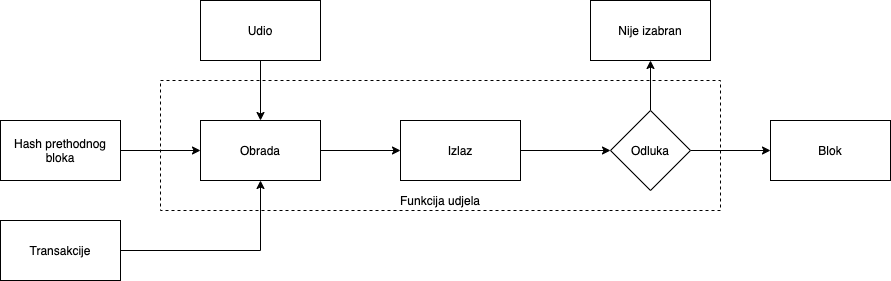
\includegraphics[width=12cm]{imgs/PoS.png}
\caption{Dokaz uloga}
\label{fig:pos}
\end{figure}

Dokaz uloga funkcionira tako da rudar može rudariti blok ovisno o količini resursa (kriptovalute) koju posjeduje, dakle ne riješava nikakvu kriptografsku slagalicu što uklanja potrebu za velikim računalnih resursima. Takvi sustavi čine većinski napad jako skupim, stoga se napadačima i ne isplati pokušavati. Takvi su sustavi također i više decentralizirani, ali potrebno je puno truda uložiti kako bi se izgradile zajednice oko takvih sustava.

\subsection{Paxos}

Paxos je obitelj konsenzusnih protokola koji osiguravaju dosljednost replika u distribuiranom sustavu nepouzdanih procesora, odnosno sustavu u kojem poslužitelji mogu zakazati. Protokol Paxos uveo je 1989. Leslie Lamport, nazvan po izmišljenom zakonodavnom sustavu konsenzusa koji se koristio na otoku Paxos u Grčkoj. Cilj Paxos algoritma je održavanje istog redoslijeda naredbi među više replika, tako da sve replike na kraju konvergiraju u istu vrijednost. To je slično slučaju kada više automobila slijedeći iste upute stiže na isto konačno odredište.

\subsection{Raft}
\label{sec:raft}
Raft je konsenzusni algoritam koji je dizajniran tako da ga je lako razumjeti. Jednak je Paxosu u toleranciji kvarova i performansama. Razlika je u tome što je razložen na relativno neovisne podprobleme i bavi se svim glavnim dijelovima potrebnim za praktične sustave na uredniji način. Kako bi se poboljšala razumljivost, Raft razdvaja ključne elemente konsenzusa, kao što su izbor vođe, replikacija zapisnika i sigurnost te provodi snažniji stupanj konherentnosti kako bi se smanjio broj stanja koja se moraju uzeti u obzir. Raft također uključuje novi mehanizam za promjenu članstva klastera,
koji koristi preklapajuće većine kako bi se zajamčila sigurnost. \cite{raft}

\begin{figure}[htb]
\centering
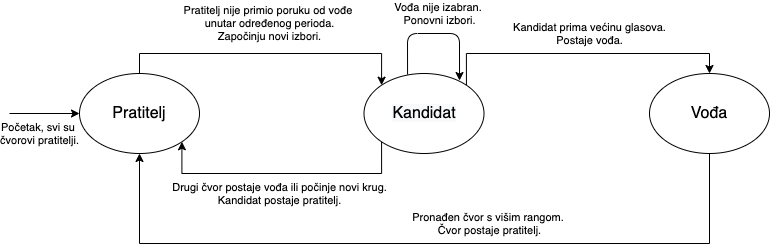
\includegraphics[width=12cm]{imgs/Raft.png}
\caption{Raft konsenzus}
\label{fig:raft}
\end{figure}

\subparagraph{Osnove}

\begin{itemize}

\item za ispravan rad mreže potreban je kvorum (većina) čvorova;

\item čvorovi mogu biti u tri stanja - vođa, kandidat za vođu ili sljedbenik;

\item vođa upravlja ažuriranjem stanja mreže. Vođa se određuje glasovanjem;

\item kada prođe vremensko ograničenje izbora (sljedbenik ne primi nikakvu komunikaciju određeno vrijeme) započinje novi izbor vođe;

\item vođa periodički šalje heartbeat poruke, kako bi zadržao autoritet nad sljedbenicima.

\end{itemize}

\subparagraph{Razlike u odnosu na Paxos}

\begin{itemize}

\item snažan vođa - Raft koristi jači oblik vodstva od ostalih konsenzusnih algoritama. Na primjer, zapisnik se šalje samo od voditelja do drugih čvorova. Ovo pojednostavljuje upravljanje repliciranim zapisnikom i čini Raft lakšim za razumijevanje;

\item izbor vođe - Raft koristi nasumične tajmere za biranje vođe. To dodaje samo malu količinu dodatnog mehanizma već otprije potrebnim mehanizmima za bilo koji algoritam konsenzusa, dok sukobe rješava jednostavno i brzo;

\item promjene članstva - Raftov mehanizam za promjene skupa čvorova u klasteru koristi novi zajedniki konsenzusni pristup gdje se većina dvije različite konfiguracije preklapa tijekom prijelaza. To omogućuje klasteru da nastavi raditi normalno tijekom promjena konfiguracije.

\end{itemize}

\section{Pametni ugovori}

Pojam pametni ugovor korišten je tijekom godina za opisivanje širokog spektra različitih stvari. Devedesetih je kriptograf Nick Szabo skovao taj pojam i definirao ga kao "skup obećanja, specificiranih u digitalnom obliku, uključujući protokole unutar kojih stranke izvršavaju ostala obećanja". Od tada se koncept pametnih ugovora razvijao,  posebno nakon uvođenja decentraliziranih blockchain platformi s izumom Bitcoina 2009. Taj pojam najčešće je povezan s Ethereum blockchainom, no kontekstu Ethereuma, taj je izraz zapravo pomalo pogrešan naziv, s obzirom na to da pametni ugovori Ethereum nisu ni jedno ni drugo. Nisu pametni niti pravni ugovori, ali termin je zapeo.
Što su onda zapravo pametni ugovori? Ethereum definira pametne ugovore u sljedećih nekoliko stavki:

\begin{itemize}

\item \textbf{računalni program} - Pametni ugovori su jednostavno računalni programi. Riječ "ugovor" u ovom kontekstu nema pravno značenje;

\item \textbf{nepromjenjiv} - Jednom postavljen, kôd pametnog ugovora ne može se mijenjati. Za razliku od tradicionalnog softvera, jedini način izmjene pametnog ugovora je postavljanje nove instance;

\item \textbf{deterministiki} - Ishod izvršenja pametnog ugovora jednak je za sve koji ga izvode, s obzirom na kontekst transakcije koja je pokrenula njegovo izvršenje i stanje blockchaina u trenutku izvršenja;

\item \textbf{kontekst Ethereumovog virtualnog stroja} - Pametni ugovori rade s vrlo ograničenim kontekstom izvršenja. Mogu pristupiti vlastitom stanju, kontekstu transakcije koja ih je pozvala i nekim informacijama o najnovijim blokovima;

\item \textbf{decentralizirano svjetsko računalo} - EVM radi kao lokalna instanca na svakom Ethereum čvoru, ali budući da sve instance EVM-a rade u istom početnom stanju i proizvode isto konačno stanje, sustav u cjelini djeluje kao jedinstveno "svjetsko računalo".

\end{itemize}

Pametni ugovori obično su napisani u programskom jeziku visoke razine, kao što je Solidity. Ali da bi se izvodili, moraju se prevesti u bajtni kod niske razine koji se izvodi u Ethereum virtualnom stroju. Jednom sastavljeni, oni se raspoređuju na Ethereum platformi pomoću posebne transakcije stvaranja ugovora, koja se identificira kao takva slanjem na adresu za stvaranje posebnog ugovora 0x0. Svaki ugovor identificiran je Ethereum adresom koja je izvedena iz transakcije stvaranja ugovora kao funkcija izvornog računa i nonce-a. Ethereum adresa ugovora može se koristiti u transakciji kao primatelj, šaljući sredstva na ugovor ili pozivajući jednu od funkcija ugovora. Za razliku od vanjskih računa, ne postoje ključevi povezani s računom stvorenim za novi
pametni ugovor. Stvaratelj ugovora, ne dobiva nikakve posebne povlastice na razini protokola (iako ih se može izričito kodirati u pametni ugovor).
Važno je da se ugovori izvršavaju samo ako ih transakcija pozove. Svi pametni ugovori u Ethereumu izvršavaju se u konačnici zbog transakcije pokrenute od vanjskog računa. Ugovor može pozvati drugi ugovor koji može pozvati treći ugovor, i tako dalje, ali prvi ugovor u takvom lancu izvršenja uvijek će biti pozvan transakcijom od vanjskog računa. Ugovori se nikad ne izvršavaju sami ili u pozadini. Ugovori učinkovito miruju sve dok transakcija ne pokrene izvršenje, bilo izravno ili neizravno kao dio lanca ugovora.  Transakcije su atomske,  ili se uspješno izvršavaju ili poništavaju.

\begin{enumerate}

\item ako se transakcija pošalje iz vanjskog računa na drugi vanjski račun, tada se bilježe sve promjene u globalnom stanju (npr. stanja računa) izvršene transakcijom;

\item ako se transakcija pošalje iz vanjskog računa na ugovor koji se ne poziva na bilo koji drugi ugovor, tada se bilježe sve promjene globalnog stanja (npr. stanja na raćunima, varijable stanja ugovora);

\item ako se pošalje transakcija iz vanjskog računa do ugovora koji samo poziva druge ugovore na način koji propagira pogreške, tada se bilježe sve promjene globalnog stanja (npr. stanja na računima, varijable stanja ugovora);

\item ako se transakcija pošalje iz vanjskog računa na ugovor koji poziva druge ugovore na način koji ne propagira pogreške, tada mogu biti zabilježene samo neke promjene u globalnom stanju (npr. stanja na računu, varijable stanja ugovora bez pogrešaka), dok se druge promjene globalnog stanja ne bilježe (npr. varijable stanja ugovora s pogreškama). Inače, ako se transakcija poništi, svi se njezini učinci (promjene stanja) vraćaju unatrag, kao da se transakcija nikada nije pokrenula. Neuspjela transakcija i dalje se evidentira kao pokušaj, a Ether potrošen na gas za izvršenje oduzima se s izvornog računa, ali inače nema drugih učinaka na ugovor ili stanje računa.

\end{enumerate}

Kao što je prethodno spomenuto, važno je zapamtiti da se kod ugovora ne može mijenjati. Međutim, ugovor se može "izbrisati", uklanjajući kod i njegovo unutarnje stanje (pohranu) s adrese, ostavljajući prazan račun. Sve transakcije poslane na tu adresu računa nakon brisanja ugovora ne rezultiraju izvršenjem koda, jer tamo više nema koda za izvršavanje. Brisanje ugovora ne uklanja povijest transakcija ugovora,  jer je sam blockchain nepromjenjiv. Također je važno napomenuti da će mogućnost biti dostupna samo ako je autor ugovora programirao pametni ugovor da ima tu funkcionalnost.
Pametni ugovori s ograničenim pristupom postavljeni na blockchainu s ograničenim pristupom, postaju sve popularniji u poslovnom svijetu. U usporedbi s neučinkovitim i skupim procesima provjere valjanosti javnih blockchaina, blockchaini s ograničenim pristupom prikladniji su za poticanje poslovne suradnje. Javni pametni ugovori nameću neizbježne opasnosti za privatnost korisnika. Stoga se u poslovnom svijetu više koriste pametni ugovori s ograničenim pristupom, a to uključuje banke, lanac opskrbe, glasanje, IoT, osiguranje, itd.

\subsection{Tokeni}

U Blockchain ekosustavu bilo koja imovina koja je digitalno prenosiva između dvije stranke naziva se "token". Tokeni na blockchainu (kriptografski tokeni) predstavljaju skup pravila, kodiranih u pametnom ugovoru - ugovoru tokena. Svaki token pripada blockchain adresi. Ti su tokeni dostupni preko virtualnog novčanika, onog koji komunicira s blockchainom i upravlja parom javno-privatnih ključeva povezanim s adresom blockchaina. Samo osoba koja ima privatni ključ za tu adresu može pristupiti odgovarajućim tokenima. Token može predstavljati na primjer imovinu, pravo pristupa ili pak glas na izborima, a vlasnik ga može prenijeti (odobriti) tako da to potpiše svojim privatnim ključem, stvarajući digitalni potpis. Valjanost i sigurnost kriptografskih tokena kontrolira pametni ugovor koji ga je stvorio zajedno s osnovnom distribuiranom glavnom knjigom i većinskim konsenzusom.
Ethereum je razvio standardizirani pametni ugovor, standard ERC-20, koji definira zajedniki popis pravila za Ethereum tokene, uključujući način na koji se tokeni prenose s jedne Ethereum adrese na drugu i kako se pristupa podacima unutar svakog tokena. Ovi relativno jednostavni pametni ugovori upravljaju logikom i održavaju popis svih izdanih tokena i mogu predstavljati bilo koju imovinu koja ima značajke zamjenjive robe.
Besplatni i otvoreni ERC-721 standard opisuje kako napraviti takozvane nezamjenjive tokene na Ethereum blockchainu. Ovo je uvelo doba složenijih obilježja tokena.  Ovaj je standard olakšao stvaranje tokena koji predstavlja bilo koju vrstu kolekcionarskih predmeta, umjetnina, vlasništva ili personaliziranih prava pristupa. Ovi nezamjenjivi tokeni imaju posebna svojstva koja token čine jedinstvenim i povezani su s identitetom određene osobe.

Tokene trenutno nije moguće prebacivati između različitih mreža, jer se izdaju pametnim ugovorima specifinim za blockchain koji njima upravljaju. Ti različiti blockchaini imaju različite standarde i nisu interoperabilni. Rješavanje tih problema moglo bi dovesti do masovnog usvajanja tokena širom tehnološkog svijeta.
\subsubsection{ERC-20}

Standard ERC-20 (Ethereum zahtjev za komentare 20,  eng.  \textit{Ethereum Request for Comments} 20), predložen od  Fabiana Vogelstellera u studenom 2015. godine, je standard tokena koji predstavlja sučelje po kojem se programiraju pametni ugovori. Pruža funkcionalnosti poput prijenosa tokena s jednog računa na drugi, dohvaćanja trenutnog stanja tokena na računu, kao i ukupne zalihe tokena dostupnih na mreži. Osim njih, ima i neke druge funkcije poput odobrenja da iznos tokena s jednog računa može potrošiti račun treće strane. Ako pametni ugovor implementira sljedeće metode i događaje, može se nazvati ERC-20 token ugovorom, a nakon primjene bit će odgovoran za praćenje stvorenih
tokena na Ethereumu:

\begin{lstlisting}
function name() public view returns (string)
function symbol() public view returns (string)
function decimals() public view returns (uint8)
function totalSupply() public view returns (uint256)
function balanceOf(address _owner) public view returns (uint256 balance)
function transfer(address _to, uint256 _value) public returns (bool success)
function transferFrom(address _from, address _to, uint256 _value) public returns (bool success)
function approve(address _spender, uint256 _value) public returns ( bool success)
function allowance(address _owner, address _spender) public view returns (uint256 remaining)
\end{lstlisting}
\begin{lstlisting}
event Transfer(address indexed _from, address indexed _to, uint256 _value)
event Approval(address indexed _owner, address indexed _spender,  uint256 _value)
\end{lstlisting}

\subsubsection{ERC-721}

Standard ERC-721 (Ethereum zahtjev za komentare 721, eng. \textit{Ethereum Request for Comments} 721), koji su u siječnju 2018. predložili William Entriken, Dieter Shirley, Jacob Evans, Nastassia Sachs, standard je nezamjenjivog tokena koji predstavlja sučelje po kojem se programiraju pametni ugovori. Pruža funkcionalnosti poput prijenosa tokena s jednog računa na drugi, dobivanjatrenutnog stanja tokena na računu, dobivanja vlasnika određenog tokena, kao i ukupne zalihe tokena dostupnih na mreži. Osim njih, on ima i neke druge funkcije poput odobrenja da iznos tokena s računa može premjestiti račun treće strane.
Ako pametni ugovor implementira sljedeće metode i događaje, može se nazvati ERC-721 ugovorom o nezamjenjivom tokenu i nakon što se jednom primijeni, bit će odgovoran za praćenje stvorenih tokena na Ethereumu.

\begin{lstlisting}
function balanceOf(address _owner) external view returns (uint256);
function ownerOf(uint256 _tokenId) external view returns (address);
function safeTransferFrom(address _from, address _to, uint256 _tokenId, bytes data) external payable;
function safeTransferFrom(address _from, address _to, uint256 _tokenId) external payable;
function transferFrom(address _from, address _to, uint256 _tokenId) external payable;
function approve(address _approved, uint256 _tokenId) external payable;
function setApprovalForAll(address _operator, bool _approved) external;
function getApproved(uint256 _tokenId) external view returns (address);
function isApprovedForAll(address _owner, address _operator) external view returns (bool);
\end{lstlisting}
\begin{lstlisting}
event Transfer(address indexed _from, address indexed _to,  uint256 indexed _tokenId);
event Approval(address indexed _owner, address indexed _approved,  uint256 indexed _tokenId);
event ApprovalForAll(address indexed _owner, address indexed _operator, bool _approved);
\end{lstlisting}

\section{Corda, Quorum i Hyperledger Fabric}

\subsection{Corda}

Corda je platforma za distribuirane glavne knjige koje se koriste za evidentiranje i obradu financijskih sporazuma. Platforma Corda podržava pametne ugovore koji odgovaraju definiciji \cite{Corda}. Corda pametni ugovor je ugovor čije je izvršenje automatizirano pomoću računalnog koda koji radi s ljudskim unosom i kontrolom, i čija su prava i obveze pravno izvršni. Pametni ugovor povezuje poslovnu logiku i poslovne podatke s povezanim pravnim osobama kako bi se osiguralo da financijski sporazumi na platformi budu ukorijenjeni vrsto u zakonu i da se mogu provoditi te da postoji jasan put u slučaju dvosmislenosti, neizvjesnosti ili spora.
Corda je specijalizirana za uporabu u reguliranim financijskim institucijama. Inspiriran je blockchain sustavima, ali bez dizajna koji čini tradicionalne blockchaine neprikladnim za mnoge financijske scenarije. Corda pruža radni okvir za izvođenje pametnih ugovora sa sljedećim ključnim aktivnostima i značajke:

\begin{itemize}

\item zapisivanje i upravljanje evolucijom financijskih sporazuma i drugih dijeljnih podataka između dvije stranke na način koji je utemeljen na postojećim pravnim konstrukcijama i kompatibilan sa postojećim i novim regulacijama;

\item koreografiranje tijeka rada između tvrtki bez središnjeg tijela;

\item konsenzus između tvrtki na razini pojedinačnih dogovora, a ne na globalnoj razini;

\item podrška uključivanju regulatornih i nadzornih čvorova promatrača;

\item validiranje transakcija isključivo između strana u transakciji;

\item podržavanje različitih mehanizama konsenzusa;

\item zapisivanje eksplicitnih veza između pravnih dokumenata i koda pametnog ugovora;

\item ograničavanje pristupa podacima u okviru sporazuma samo onima koji su izričito s pravom ili logički privilegirani na to.

\end{itemize}

Te značajke doprinose dizajnu platforme prikladne za upotrebu u složenim  financijskim uslugama. Ovaj dizajn ne koristi izvorne kriptovalute i ne nameće globalno ograničenje brzine transakcije.

Glavna značajka Corda koncepta je \textbf{objekt stanja}, koji je zapravo digitalni dokument koji zapisuje postojanje, sadržaj i trenutno stanje sporazuma između dvije ili više stranaka. U Cordi se ažuriranja primjenjuju pomoću transakcija koje troše postojeće objekte stanja i proizvode nove objekte stanja. 

Postoje dva aspekta konsenzusa:

\begin{enumerate}

\item \textbf{valjanost transakcije}: stranke mogu biti sigurne da je predložena transakcija valjana tako da izvrši kod ugovora uspješno i da ima sve valjane potpise. Ovo također mora vrijediti i za sve transkacije na koje se ova transakcija referira;

\item \textbf{jedinstvenost transakcije}: stranke mogu biti sigurne da je transakcija u pitanju jedinstveni potrošač svih njenih ulaznih stanja. Odnosno, ne postoji nijedna druga transakcija za koju je prethodno postignut konsenzus (valjanost i jedinstvenost), koja troši bilo koje od istih stanja. Stranke se mogu dogovoriti o valjanosti transakcija samostalnim pokretanjem istog koda ugovora i logike validacije. Međutim, konsenzus oko jedinstvenosti zahtijeva unaprijed određenog promatrača,  koji će u mnogim sluajevima morati biti neovisan.

\end{enumerate}

\subsection{Quorum}

Quorum je razvila tvrtka J.P. Morgan kao inaicu Ethereum blockchaina s ograničenim pristupom. Ethereum je javni blockchain bez ograničenog pristupa koji se koristi za izradu decentraliziranih aplikacija unutar različitih domena. Ima podršku za Turing-potpune pametne ugovore i stoga se može koristit za izradu aplikacija opće namjene.  Iako je javan i bez ograničenja pristupa, sigurnost Ethereuma proizlazi iz Dokaz izvršenog rada konsenzusnog algoritma i interne kriptovalute Ether. Quorum uključuje sljedeće ključne promjene u odnosu na Ethereum:

\begin{itemize}

\item ograničeno sudjelovanje - stavlja restrikciju na sudjelovanje u blockchain mreži samo onim ččvorovima kojima je to dopušteno. Samo je njima dopušteno povezivanje na Quorum blockchain, provjeravanje transakcija, pokretanje pametnih ugovora i održavanje glavne knjige;

\item konsenzusni algoritmi - Quorum prema zadanim postavkama koristi Raft i Istanbulski BFT konsenzus. Ova dva algoritma pružaju zamjenu za Ethereumov PoW. Dok PoW štiti javni blockchain postepeno uvodeći težinu u kriptografsku slagalicu, potpuno je nepotrebno i rastrošno (velika potrošnja energije) za sustav ograničenog pristupa gdje si stranke međusobno vjeruju. Raft i IBFT algoritmi dovode do bržeg konsenzusa i pružaju trenutnu konačnost transakcije, čineći ih prikladan izbor za PB. Quorum također podržava lako promjenjivu arhitekturu u koju se po potrebi može uključiti drugačija implementacija konsenzusa;

\item privatnost - jedan od ciljeva dizajna Quoruma. Dozvoljava manjem dijelu konzorcija da vrše transakcije između sebe bez da ih javno iznose ostatku konzorcija. Privatnost u Quorum je omogućena podjelom veće javne glavne knjige na javnu i privatnu. Javna glavna knjiga je vidljiva svim čvorovima u mreži, a privatna samo onima koji vrše transkacije međusobno. Samo hash privatne transakcije je vidljiv na javnoj glavnoj knjizi, ali samo stranke između kojih je izvršena transakcija imaju ključ s kojim mogu pregledati transakciju. Također se i pametni ugovori mogu dijeliti na privatan način, između stranaka koje međusobno vrše transakcije;

\item ukidanje cijena transakcija - Quorum je eliminirao dodavanje troškova transakcijama pomoću \textit{gas}-a. Stoga, Quorum nema troškova povezanih s izvođenjem transakcija na Quorum mreži. S obzirom da je Quorum kod "forkan" od Ethereuma, korištenje gas-a postoji ali je namješteno na 0. Gas je korišten u Ethereum mreži za plaćanje izvođenja transakcija (koristi se ether kriptovaluta) kako bi se incentivizirali rudari i kako bi se Ethereum mreža zaštitila od spam-a i DDoS napada.

\end{itemize}

\subsection{Hyperledger Fabric}

Mnogi PB-i trpe zbog mnogih ogranienja, koji esto proizlaze iz njihovih predaka - javnih blockchaina, ili iz upotrebe arhitekture "poredaj-izvrši" (eng. order-execute):

\begin{itemize}

\item konsenzus je vrsto kodiran unutar platforme, što je u suprotnosti s ustaljenim shvaćanjem da ne postoji jednoznačni (BFT) konsenzus protokol;

\item model povjerenja validacije transakcija je određen konsenzusnim protokolom i ne može se prilagoditi zahtjevima pametnog ugovora;

\item pametni ugovori moraju biti pisani na fiksan, nestandardan ili specifičan za domenu jezik, što ometa široko usvajanje i može dovesti do pogrešaka prilikom programiranja;

\item slijedna izvedba svih transakcija od svih čvorova ograničava performanse, te su potrebne komplicirane mjere kako bi se spriječio DDoS napad;

\item transakcije moraju biti deterministike, što je teško ostvariti programski;

\item svaki pametni ugovor se izvršava na svim čvorovima, što je u suprotnosti povjerljivosti i zabranjuje širenje koda ugovora i stanje podskupu čvorova.

\end{itemize}

U ovom radu opisujemo Hyperledger Fabric ili jednostavno Fabric, blockchain
platformu otvorenog koda koja prevladava ta ograničenja. Fabric je jedan od projekata Hyperledgera u okviru pokroviteljstva zaklade Linux. Fabric se koristi u više od 400 prototipova, dokaza o konceptu, produkcijskim raspodijeljenim glavnim knjigama i u različitim industrijama. Ovi slučajevi korištenja uključuju, ali nisu ograničeni na područja kao što su rješavanje sporova, trgovinska logistika, devizna mreža, sigurnost hrane, upravljanje ugovorima, dijamantna provenijencija, upravljanje bodovima, trgovanje niskom likvidnosti, upravljanje identitetima i namirba putem digitalne valute.

Fabric uvodi novu blockchain arhitekturu s ciljem elastičnosti, fleksibilnosti, skalabilnosti i povjerljivosti. Dizajniran kao modularni i proširivi PB, Fabric je prvi blockchain sustav koji podržava izvršavanje distribuiranih aplikacija napisanih u standardnim programskim jezicima, na način koji omogućuje njihovo dosljedno izvršavanje preko mnogih čvorova, ostavljajući dojam izvršenja na jednom globalno distribuiranom blockchain
računalu. To Fabric čini prvim distribuiranim operativnim sustavom za PB.
Hyperledger Fabric uvodi i još jedan imbenik modularnosti i fleksibilnosti, a to su takozvani kanali. Kanali omogućavaju sudionicima stvarnje virtualnih grupa i održavanje neovisnih glavnih knjiga koje su nevidljive drugim kanalima u mreži. Kanali pružaju fleksibilnost poslovnom konzorciju da sigurno dijeli informacije samo s relevantim strankama.
Arhitektura Fabric slijedi novu "izvrši-poredaj-validiraj" paradigmu za distribuirano izvršavanje nepovjerljivog koda u nepouzdanom okruženju. Tok transakcije razdvaja na tri koraka koji se mogu izvoditi na različitim entitetima u sustavu:

\begin{enumerate}

\item izvršavanje transakcije i provjera njezine ispravnosti i valjanosti;

\item redoslijed (eng.  \textit{ordering}) putem konsenzusnog protokola, bez obzira na semantiku transakcije;

\item validacija transakcije po pretpostavkama specifičnim aplikaciji, što također sprječava tzv.  \textit{race conditions}.

\end{enumerate}

Ovaj dizajn radikalno odstupa od paradigme \textit{order-execute} tako da Fabric obično izvršava transakcije prije postizanja konačnog dogovora o njihovom redoslijedu. Kombinira dva pristupa repliciranju, pasivni i aktivni.
Prvo, Fabric koristi pasivnu ili primarno-sigurnosnu replikaciju kao što se čestonalazi u distribuiranim bazama podataka, ali s posredničkim softverom koji procesuira ažuriranja asimetrično i u nepouzdanoj okolini s Bizantskim pogreškama. U Fabricu svaka transakcija se izvršava (odobrava) samo na podskupu čvorova (eng. peer), što dopušta paralelno izvršavanje i rješava potencijalni nedeterminizam, oslanjajući se na BFT replikaciju "izvrši-provjeri" (eng. execute-verify). Fleksibilna politika odobravanja transakcija određuje koji peer-ovi ili koliko njih treba jamčiti za ispravno izvršenje zadanog pametnog ugovora.
Drugo, Fabric uključuje aktivnu replikaciju u smislu da učinci transakcije na stanje glavne knjige pišu se tek nakon postizanja konsenzusa o ukupnom redoslijedu među njima, u koraku determinističke validacije koji izvršava svaki peer pojedinačno. Ovo omogućava Fabricu da se prilagodi pretpostavkama povjerenja specifičnih za aplikaciju.
Štoviše, ordering ažuriranja stanja delegirana je modularnoj komponenti radi konsenzusa, koja je bez stanja i logički odvojena od peerova koji izvršavaju transakcije i održavaju glavnu knjigu. Zbog konsenzusa koji je modularan, njegova se primjena može prilagoditi pretpostavkama o povjerenju određenog razvoja. Iako je moguće koristiti blockchain peer-ove i za provođenje konsenzusa, razdvajanje dviju uloga dodaje fleksibilnost i omogućuje osloniti se na dobro uspostavljene alate za otpornost na kvarove
(eng. Crash Fault Tolerance, skr. CFT).
Sve u svemu, ovaj hibridni replikacijski dizajn koji miješa pasivnu i aktivnu replikaciju u bizantskom modelu i paradigma \textit{execute-order-validate} predstavljaju glavnu inovaciju u arhitekturi Fabrica. Oni rješavaju prethodno spomenute probleme i omugu ćuju da Fabric bude skalabilni sustav za PB koji podržava fleksibilne pretpostavke povjerenja. Da bi implementirao ovu arhitekturu, Fabric sadrži modularne građevne blokove za svaku od sljedećih komponenata:

\begin{itemize}

\item usluga poravnanja transakcija atomski emitira ažuriranja stanja peer-ovima i uspostavlja konsenzus na redoslijed transakcija;

\item usluga članstva (eng. Membership service provider, skr. MSP) je odgovorna za pridruživanje kriptografskih identiteta peer-ovima. Zapravo održava ograničenja pristupa unutar Fabrica;

\item opcionalna \textit{peer-to-peer gossip} usluga širi izlaze blokova svim peer-ovima;

\item pametni ugovori u Fabricu izvršavaju se unutar kontejnera, izolirani. Mogu biti napisani u standardnim programskim jezicima, ali nemaju direktan pristup stanju glavne knjige;

\item svaki peer lokalno održava glavnu knjigu u formi blockchaina na koji je moguće samo dodavati blokove i kao snapshot posljednjeg stanja u "ključ-vrijednost" pohrani.

\end{itemize}

\subsection{Usporedba}

U ovoj sekciji usporedit ću tri prethodno navedene izvedbe blockchaina s ograničenim pravom pristupa. Provest ću analizu svake izvedbe prema tome kako implementiraju konsenzus, pametne ugovore, autentifikaciju i autorizaciju i prema propusnosti transakcija.

\subsubsection{Konsenzus}

U blockchain mreži, tijekom obrade bloka, čvorovi obavljaju određene aktivnosti, kao što su sudjelovanje u provjeri autentičnosti i provjeri transakcija, komunikacija preko mreže i izgradnja povjerenja unutar blockchain sustava bez uplitanja središnjeg autoriteta. Uvijek postoji rizik da se pojedini čvorovi mogu ponašati zlonamjerno ili djelovati protiv osnovnog cilja i pokušati srušiti komunikaciju u mreži. Da bi se osigurala kontinuirana usluga koja pruža dostupnost, povjerljivost, integritet, i pristupačnost potreban je siguran mehanizam da bi svi čvorovi sudionici postigli globalni dogovor koje
informacije trebaju biti dodane blockchainu. Ovaj postupak je poznat kao konsenzus.
Hyperledger Fabric u prvoj verziji koristi konsenzus protokol Apache Kafka. Kafka nije tradicionalni konsenzusni protokol, nego je "\textit{publish-subscribe}" rješenje. Kafka koristi isti "vođa i sljedbenik" koncept kao i Raft kao što je vidljivo na slici 2.4, u kojem su transakcije (Kafka koristi pojam "poruka") replicirane od čvora vođe do čvorova sljebenika. Od verzije 2.0 Fabric koristi Raft konsenzus prethodno opisan u poglavlju \ref{sec:raft}.

\begin{figure}[htb]
\centering
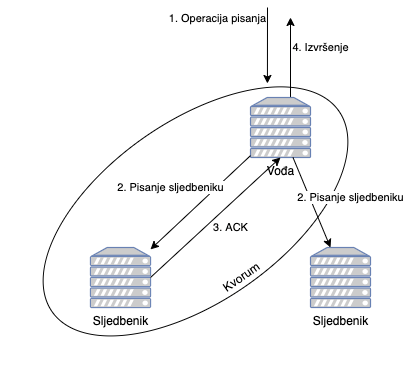
\includegraphics[width=12cm]{imgs/Kafka.png}
\caption{Kafka konsenzus}
\label{fig:kafka}
\end{figure}

Quorum po zadanim postavkama koristi Raft za toleranciju pada sustava i Istanbulski BFT za toleranciju Bizantske pogreške. Istanbulski BFT konsenzus je konsenzus u 3 faze: pred-priprema, priprema i izvršenje. Ovaj konsenzus sustav može tolerirati da jedna trećina svih čvorova u mreži bude neispravan, a opet osigurava konačnost transakcije. Čvorovi koji su izabrani kao "validatori" bloka odabiru "predlagača" za predlaganje novog bloka u konsenzusnom krugu. Predlagatelj će tada predložiti novi blok i emitirati ga zajedno s porukom "pred-priprema". Po primitku "pred-priprema" poruke predlagatelja, validatori ulaze u stanje "pred-pripremljeno", a zatim emitiraju "priprema" poruku. Ovaj korak želi osigurati da svi validatori rade u istom slijedu i istom krugu. Nakon primanja poruke "priprema" od dvije trećine mrežnih čvorova, validator ulazi u stanje "pripremljeno", a zatim emitira "izvrši" poruku. Ovaj korak služi tome da se obavijeste peer-ovi da validator prihvaća predloženi blok i da će ga dodati u lanac. Na kraju, validatori čekaju da dvije trećine poruka "izvrši" uđu u stanje "izvršeno" i zatim umetnu blok u lanac.

\begin{figure}[htb]
\centering
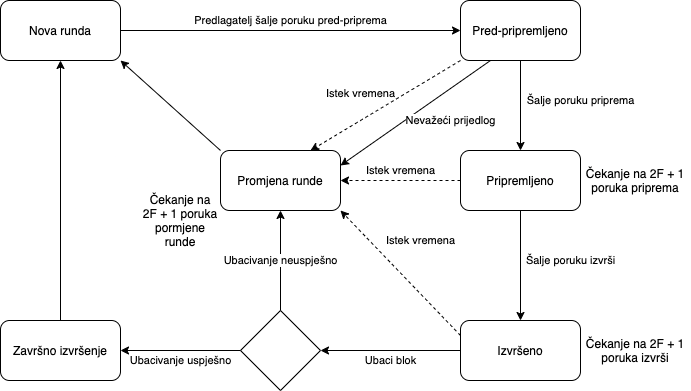
\includegraphics[width=12cm]{imgs/IBFT.png}
\caption{IBFT}
\label{fig:ibft}
\end{figure}

Corda ima zamjenjivu uslugu jedinstvenosti. To služi tome da se poboljša privatnost, skalabilnost, kompatibilnost pravnog sustava i algoritamska agilnost. Jedna usluga može biti sastavljena od mnogih međusobno nepovjerljivih čvorova koji se koordiniraju preko BFT algoritma ili može biti vrlo jednostavna, poput jednog stroja. U nekim slučajevima, kada ažuriranje stanja zahtijeva potpise svih relevantnih strana, možda uopće ne treba usluga jedinstvenosti. Konsenzus oko valjanosti transakcije provodi se samo između stranaka između kojih obavljena ta transakcija. Stoga se podaci dijele samo s tim stranama. Ostale platforme uglavnom postižu konsenzus na razini glavne knjige. Dakle, bilo koji akter u sustavu Corda vidi samo podskup ukupnih podataka kojima upravlja sustav u cjelini. Dio podataka zapisan je u glavnu knjigu ako su barem dva aktera u sustavu konsenzusni o njegovom postojanju i pojedinostima i dopuštaju se proizvoljne kombinacije aktera da sudjeluju u postupku konsenzusa za bilo koji podatak.

\begin{figure}[htb]
\centering
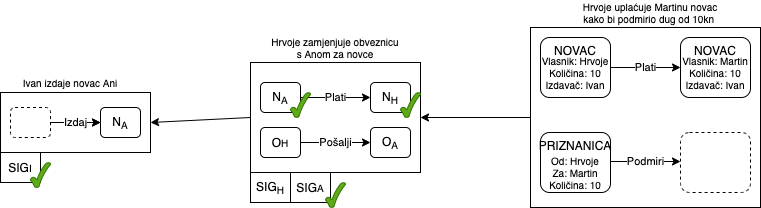
\includegraphics[width=12cm]{imgs/Validity consensus.png}
\caption{Valjanost}
\label{fig:validity}
\end{figure}

Prilikom provjere predložene transakcije, određena stranka ne mora imati svaku transakciju u lancu transakcija koju trebaju provjeriti. U tom slučaju,  može zatražiti transakcije kojih nema od predlagatelja transakcija. Predlagatelji transakcije uvijek će imati potpuni transakcijski lanac, budući da bi to zatražili prilikom provjere transakcije koja je stvorila predložena ulazna stanja.

\begin{figure}[htb]
\centering
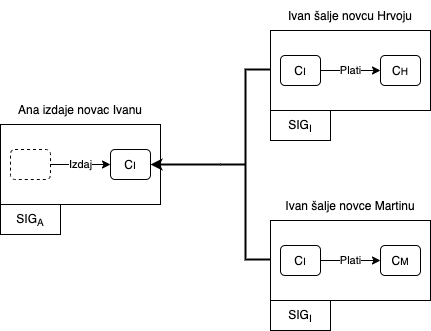
\includegraphics[width=12cm]{imgs/Uniqueness consensus.png}
\caption{Jedinstvenost}
\label{fig:uniqueness}
\end{figure}

Valjani prijedlog transakcije također mora postići konsenzus jedinstvenosti. Konsenzus jedinstvenosti je uvjet da ni jedno od ulaznih stanja predložene transakciju nije već konzumirano u drugoj transakciji. Ako je jedan ili više ulaza već konzumirano u drugojvtransakciji, to je poznato kao dvostruka potrošnja, a prijedlog transakcije smatra se nevažećim. Konsenzus jedinstvenosti omogućuju bilježnici (eng. \textit{Notaries}) koji vrše provjeru dvostruke potrošnje.

\subsubsection{Pametni ugovori}
Pametni ugovor u Corda sustavu je sporazum čiju je izvedbu moguće automatizirati računalnim kodom i čija prava i obveze, navedene u takozvanoj legalnoj prozi (eng. legal prose), su legalno provedive. Pametan ugovor u Cordi ima tri ključna elementa, a to je izvršni kod, objekte stanja i naredbe. Izvršni kod uglavnom provjerava promjene objekata stanja u transakcijama. Objekti stanja su podaci koji bilježe postojanje, sadržaj i trenutno stanje sporazuma između dvije ili više strana i rade kao ulaz ili izlaz transakcije. Naredbe su dodatni podaci koji su uključeni u transakcije. Oni uglavnom opisuju što se događa i govore izvršnom kodu na koji način verificirati transakcije. 

Quorum je blockchain s ograničenim pravom pristupa implementiran na Ethereum protokolu. Osnovna ideja koja stoji iza Quoruma je korištenje kriptografije kako bi se spriječili svi osim onih koji sudjeluju u transakcijama od gledanja osjetljivih podataka. Rješenje uključuje jedan zajedniki blockchain i kombinaciju softverske arhitekture pametnih ugovora i modifikacija Ethereuma. Arhitektura pametnih omogućuje segmentaciju privatnih podataka. Izmjene Ethereum izvornog koda uključuju modifikacije u procesu prijedlaganja bloka i procesu validacije. Proces validacije je modificiran tako da svi čvorovi potvrđuju javne transakcije i bilo koje privatne transakcije u kojima sudjeluju izvršenjem koda pametnog ugovora povezanog s transakcijama. Za ostale privatne transakcije, čvor će jednostavno preskoiti postupak izvršavanja koda ugovora.

Hyperledger Fabric često izmjenjuje izraze pametni ugovor i lančani kod (eng. \textit{Chaincode}). Općenito, pametni ugovor definira transakcijsku logiku koja kontrolira životni ciklus poslovnog objekta koji se nalazi u globalnom stanju. Zatim se pakira u lančani kod koji se zatim raspoređuje u blockchain mrežu. Pametni ugovor može opisati gotovo beskonačan niz slučajeva poslovne upotrebe koji se odnose na nepromjenjivost podataka u višeorganizacijskom donošenju odluka. Posao programera pametnih ugovora je preuzeti postojeći poslovni proces koji može regulirati financijske cijene ili uvjete isporuke i izraziti ga kao pametni ugovor u programskom jeziku kao što su JavaScript, Go ili Java.

\subsubsection{Autentifikacija i autorizacija}
Ethereum razlikuje dvije vrste računa koji se koriste za transakcije, a to su računi ugovora i vanjski računi. Svaki račun ima svoje stanje, a globalno stanje mreže je skup svih stanja računa. računi u Quorumu, koji je izveden iz Ethereuma, imaju potpuno istu strukturu. Quorum je blockchain s ograničenim pravom pristupa, a osigurava da u razmjeni poruka mogu sudjelovati samo ovjereni čvorovi. Autentifikacija čvora pošiljatelja oslanja se na autentifikaciju na temelju ključa koristeći ECDSA (eng. Elliptic Curve Digital Signature Algorithm) potpis - svakom je korisniku dodijeljen par asimetričnih ključeva generiranih pomoću eliptine krivulje secp256k1 i sadrže popis drugih javnih ključeva čvorova u mreži.  \cite{johnson2001elliptic} ECDSA omogućava primatelju izvlačenje javnog ključa pošiljatelja iz potpisa poruke koji uspoređuje s listom javnih ključeva drugih čvorova u mreži. Ako se ključ podudara, čvor je autentificiran, u protivnom se odbija veza. Opcionalno se može omogućiti TLS koji zahtijeva uzajamnu provjeru autentičnosti klijenta ili poslužitelja. Dostupno je nekoliko načina rada: TOFU, CA i bijela lista (eng. whitelist) (TOFU i CA kombinirano). Ključevi za identitet i TLS mogu sem ponovno iskoristiti.

\begin{itemize}

\item TOFU (eng.  \textit{trust-on-first-use}) - samo prvi čvor koji se poveže s identifikacijom određenog host-a moći će se povezati samo kao isti host u budućnosti. Oslanja se na provjeru autentičnosti na temelju ključa;

\item CA (eng.  \textit{certificate authority}) - samo čvorovi s ispravnim certifikatom i lancom povjerenja se mogu povezati. Oslanja se na provjeru autentičnosti na temelju certifikata;

\item WHITELIST - samo čvorovi koji su se prethodno povezali s tim čvorom i dodani su u datoteku "poznati klijenti" (eng.  \textit{knownclient}) moći će se povezati.  Oslanja se na provjeru autentičnosti na temelju ključa.

\end{itemize}

Autentifikacija incijatora transakcije, slično Ethereumu, oslanja se na autentifikaciju na temelju ključa pomoću ECDSA potpisa koji se koriste za potvrdu da je pošiljatelj vlasnik računa s kojeg transakcija proizlazi. Quorum uvodi koncept privatnosti transakcija i razlikuje javne transakcije od privatnih transakcija. Javne transakcije su identične Ethereum transakcijama i dostupna svima u mreži, dok je privatna transakcija dostupna ograničenom broju čvorova koje definira pošiljatelj. Uz svaku transakciju povezana je lista kontrole pristupa koja sadrži javne ključeve autoriziranih čvorova.
U Hyperledger Fabric-u postoje dvije vrste transakcija opisane u nastavku:

\begin{itemize}

\item transakcija postavljanja (eng. \textit{deploy transaction}) - stvara novi chaincode i prima program kao parametar. Kada se ta transakcija uspješno izvrši, chaincode je instaliran na blockchain;

\item transakcija pobude (eng. \textit{invoke transaction}) - izvodi operaciju u kontekstu prethodno postavljnog chaincode-a. Ta transakcija odnosi se na chaincode i na jednu od funkcija koju chaincode nudi.

\end{itemize}

Servis članstva (eng. Membership service provider, skr. MSP) nudi apstrakciju arhitekture lanstva. Upravlja provjerom autentičnosti i autorizacijom u mreži, a podijeljen je na različite razine:

\begin{itemize}

\item MSP mreže - definira sudionike mreže putem popisa MSP-a organizacija i pruža njihovu autorizaciju, naprimjer ovlaštenje za stvaranje kanala;

\item MSP kanala - definira administrativna i participativna pravan na razini kanala. Svaka organizacija koja sudjeluje u kanalu mora imati definirani MSP. Peer-ovi i orderer-i u kanalu dijele isti popis MSP-ova, stoga mogu ispravno autentificirati sudionike kanala;

\item lokalni MSP (orderer-i, peer-ovi, klijenti) - omogućava korisniku da se autentificira u svojim transakcijama kao član kanala, ili kao vlasnik određene uloge (autorizacija) u sistemu (npr. administrator organizacije). Lokalni MSP su definirani za klijente i za čvorove (peer-ovi i orderer-i).

\end{itemize}

Hyperledger Fabric pruža opciju korištenja predefiniranog tijela za izdavanje certifikata koje se može koristiti za generiranje certifikata i ključeva. Međutim može se zamijeniti za bilo koji CA koji može generirati ECDSA certifikate. Protokol za provjeru izvornosti poruke koristi certifikat X.509 na temelju ECC-a \cite{lagarde2019security} i opcionalne TLS certifikate. Za provjeru autentičnosti pošiljatelja poruke od strane kanala, mora predstaviti certifikat s provjerljivim putem do točno jednog od korijena povjerljivog certifikata.  Da bi se pridružio kanalu, novi čvor mora poslati zahtjev za potpisivanje certifikata na jedan od kanalovih korijenskih ili posredničkih CA-ova. Nadalje, mora konfigurirati svoj lokalni MSP sa sljedećim informacijama:

\begin{itemize}

\item korijen povjerljivog certifikata;

\item (opcionalno) posrednički CA certifikati;

\item certifikat MSP administratora;

\item popis opoziva certifikata koji odgovaraju prethodno navedenim CA-ovima (korijenskim ili posredničkim);

\item TLS korijen povjerljivog certifikata;

\item (opcionalno) posrednički TLS CA;

\item (opcionalno) lista organizacijskih jedinica koje član tog MSP-a mora sadržavati u svom certifikatu.

\end{itemize}

Kanal u Fabric-u po želji definira određene uloge unutar kanala pomoću kontrole pristupa zasnovane na atributima (eng. \textit{Attribute-Based Access Control}, skr. ABAC) koja se temelji na atributima identiteta sadržanih u certifikatima. Transakcije postavljanja ne zahtijevaju posebno odobrenje. Unutar kanala svi imaju pristup transakcijama i ne postoje sheme autorizacije za pristup određenoj transakciji, transakcije se tretiraju kao uobičajene poruke i stoga se provjera autentičnosti pošiljatelja transakcija obrađuje slično autentifikaciji pošiljatelja poruke. Autorizacijska shema odobrenja transakcija oslanja se na liste kotrole pristupa: da bi transakcija bila odobrena, mora se odobriti prema politici odobrenja pozvanog chaincode-a. Tok operacije odobrenja prikazan na slici \ref{fig:fabrictxflow} je sljedeći:

\begin{enumerate}

\item klijent kreira transakciju i šalje je odobravajućim peer-ovima koje odabere;

\item odobravajući peer simulira transakciju i proizvodi odobravajući potpis;

\item klijent prikuplja odobrenje transakcije i emitira ga putem servisa poravnavanja;

\item servis poravnavanja dostavlja transakciju peer-ovima.

\end{enumerate}

\begin{figure}[htb]
\centering
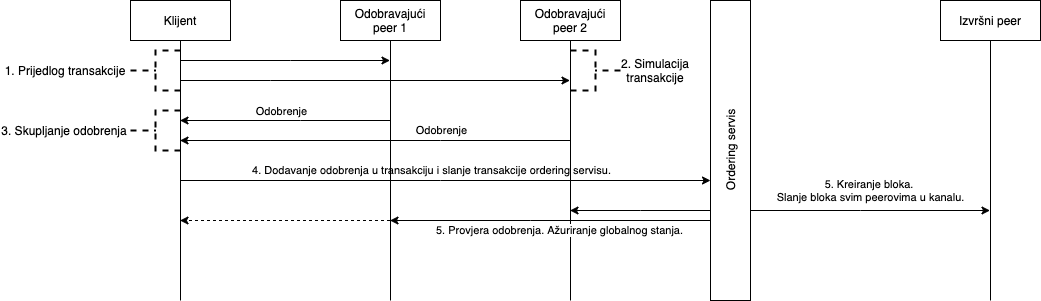
\includegraphics[width=15cm, height=6cm]{imgs/Tx Flow.png}
\caption{Hyperledger Fabric tijek transakcija}
\label{fig:fabrictxflow}
\end{figure}

U Cordi, zona kompatibilnosti označava mrežu koja ima ograničen pristup. Corda mreža ima četiri vrste CA:

\begin{itemize}

\item korijenski CA;

\item vratar CA - ponaša se kao posrednički CA;

\item CA čvora - svaki čvor služi kao svoj CA u izdavanju podređenih certifikata koje koristi za potpisivanje svojih ključeva identiteta i TLS certifikata;

\item CA legalnih identiteta - "dobro poznati" legalni identiteti čvorova, osim potpisivanja transakcija, mogu izdavati certifikate za povjerljive legalne identitete.

\end{itemize}

Cordin dizajn integrira provjeru autentičnosti temeljenu na certifikatima koristeći digitalne potipse kako bi se provjerila autentičnost pošiljatelja poruke. Čvorovi posjeduju TLS certifikate i certifikate identiteta. Kada čvor primi zahtjev za povezivanjem, provjerava lanac povjerenja TLS certifikata i certifikata identiteta. Potpisi oba certifikata u lancu moraju biti valjani skroz do korijenskog CA. Da bi se čvor priključio mreži potrebno je proći kroz sljedeće korake:

\begin{enumerate}

\item novi čvor mora posjedovati korijenski CA u svojoj pohrani povjerenja, adresu vratara i kartu mreže;

\item čvor se mora prijaviti sa svojim certifikatom na vratara podnošenjem zahtjeva za potpisivanje certifikata da bi dobio CA certifikat čvora;

\item iz CA certifikata čvora, čvor stvara i potpisuje još dva certifikata, TLS certifikat i certifikata za čvorov "dobro poznati" identitet;

\item konačno, čvor gradi zapis podataka o čvoru koji sadrži njegovu adresu i dobro poznati identitet te ga registrira s uslugom karte mreže.

\end{enumerate}

\begin{figure}[htb]
\centering
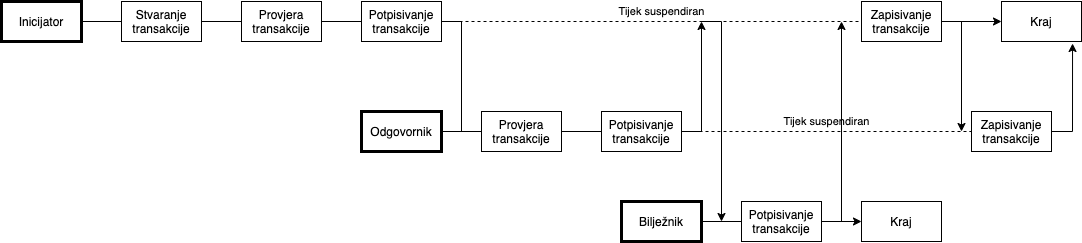
\includegraphics[width=15cm]{imgs/Corda flow.png}
\caption{Corda tijek transakcija}
\label{fig:cordaflow}
\end{figure}

Corda specificira akcije koje je čvoru dopušteno poduzeti koristeći ABAC - tipovi identiteta su definirani u certifikatu. Tipovi mogu biti sljedeći:

\begin{itemize}

\item vratar (eng.  \textit{doorman});

\item karta mreže (eng.  \textit{network map});

\item identitet servisa (eng. \textit{service identity});

\item autoritet certifikata čvora (eng.  \textit{node certificate authority});

\item sigurnost transportnog sloja (eng.  \textit{transport layer security});

\item "dobro poznati" legalni identitet (eng. \textit{well-known legal identity});

\item povjerljivi legalni identitet (eng.  \textit{confidential legal identity}).

\end{itemize}

U suprotnosti s mnogim blockchain platformama s ograničenim pravom pristupa, u Cordi sve transakcije su privatne što znači da su djeljene samo između dionika, i autorizaciju za pozivanje transakcije daje bilježnik. Da bi transakcija bila valjana, sva ulazna stanja moraju se prvo prebaciti na istog bilježnika. To se radi pomoću posebne transkacije za promjenu bilježnika koja proizvodi izlazno stanje slično ulaznom stanju,  ali prebačeno na novog bilježnika. 
Udaljena autentifikacija korisnika podržana je autentifikacijom putem lozinke kojom se upravlja na razini čvora. Opcionalno se može postaviti provjera autentičnosti klijenta temeljem certifikata pomoću TLS-a. Programski sučelje čvora potupuno je izloženo udaljenim pozivima. Ovlaštenje za upotrebu Corda udaljenog programskog sučelja koristi popise sposobnosti. Udaljeni korisnik posjeduje popis sposobnosti po udaljenom čvoru kojem pristupa. Dakle, metode koje udaljeni korisnik smije pozivati, ovise o autorizaciji koja mu je odobrena.

\subsubsection{Propusnost transakcija}

Propusnost transakcija je brzina kojom su valjane transakcije postavljene na blockchain u definiranom vremenskom periodu. Kao što se vidi na slici \ref{fig:usporedba} koja prikazuje mjerenja od \citep{9411380}, Hyperledger Fabric je najbolji izbor za izgradnju blockchaina koji treba podnijeti veliki broj transakcija. Doduše, ove analize napravljene su pomoću alata za testiranje koje su razvile tvrtke koje stoje iza samih platformi te bi se to moglo smatrati nedostakom ove analize. Analiza bi bila efikasnije i više "fer" da postoji univerzalni alat kojim je moguće provesti analizu nad svim navedenim blockchain platformama.

\begin{figure}[htb]
\centering
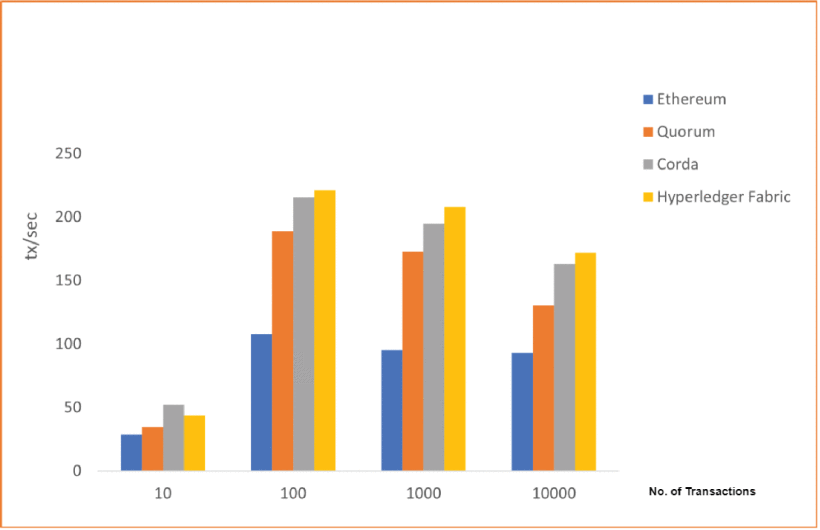
\includegraphics[width=13cm, height=7cm]{imgs/monra10-CSDE92-large.png}
\caption{Usporedba propusnosti transakcija}
\label{fig:usporedba}
\end{figure}



Fabric, razvijen od strane Linux fundacije u sklopu multi-projekta otvorenog koda je radni okvir koji sam odlučio koristiti za implementacijski dio ovoga rada. Analiza propusnosti transakcija odrađena je od strane \citep{9411380} između Ethereum, Quorum, Corda i Hyperledger Fabric platforme. Možemo primjetiti da Fabric nadmašuje Quorum i Ethereum s velikom razlikom, ali samo nešto bolje od Corde. Fabric ima nisku latenciju obrade transakcija u usporedbi s ostalim blockchainima s ograničenim pravom pristupa. Stoga je ova platforma sposobna također pružiti i bolju propusnost transakcija. Njihova eksperimentalna opažanja otkrivaju da Hyperledger Fabric ima bolje rezultate od ostalih platformi zbog svog jednostavnog i uinkovitog modularnog pristupa konsenzusu.

\chapter{Implementacija}
Implementacijski dio ovog rada odradio sam koristeći Hyperledger Fabric radni okvir.  Ovaj radni okvir omogućava da sustav koji želimo napraviti prilagodimo potrebi aplikacije vrlo detaljno. Od određivanja uloga korisnika sustava do same poslovne logike. U Fabricu svaki čvor je pokrenut kao Docker kontejner (eng. \textit{container}). Docker je set "platforma kao servis" (eng. \textit{Platform as a Service,} skr. PaaS) proizvoda koji koriste virtualizaciju na razini operativnog sustava kako bi dostavili softver u pakiranjima koji se zovu kontejneri (eng. container). Kontejneri su odvojeni jedni od drugih, ali skupa rade na istoj mreži. Datoteka koja služi za definiranje konfiguracije Docker-a je \textit{docker-compose.yaml}. U ovoj datoteci definirani su kontejneri i mreža kojoj su pridruženi i njihove varijable okruženja. Pokreće se naredbom \textit{docker-compose} kojoj se pridodaje putanja do \textit{docker-compose.yaml}datoteke.
Implementirao sam primjer dodjeljivanja hipotetskih bodova za menzu studentima i dodjeljivanje rektorovih nagrada u obliku virtualnih tokena. Bodovi za menzu predstavljeni su tokenom koji slijedi ERC-20 standard, što znači da je token "zamjenjiv" (eng. \textit{fungible}), a tokenom koji slijedi ERC-721 standard predstavljene su rektorove nagrade, a takav token je "nezamjenjiv" (eng. \textit{non-fungible}).

Direktorij u kojem se nalaze izvršne datoteke potrebne za pokretanje Fabric mreže je "bin" direktorij unutar "network" direktorija. U "bin" direktoriju nalaze se sljedeće datoteke:

\begin{itemize}
\item \textit{peer} - ova datoteka služi kao naredba preko komandne linije i dijeli se na više podnaredbi:
	\begin{itemize}
	\item \textit{peer node} - naredba omogućuje administratoru da pokrene peer čvor, resetira sve kanale kojima je peer član do genesis (nultog) bloka ili vrati kanal na zadani broj bloka.
	\item \textit{peer channel} - naredba omogućuje administratorima 			izvođenje operacija povezanih s kanalom na peer-u, poput pridruživanja peer-a kanalu ili popisa kanala kojima je peer pridružen.
	\item \textit{peer chaincode} - naredba omogućuje administratorima izvođenje operacija povezanih s lančanim kodom, poput instaliranja, instanciranja, pozivanja, pakiranja, postavljanja upita i nadogradnje lančanog koda.
	\item \textit{peer lifecycle chaincode} - podnaredba omogućuje administratorima da koriste životni ciklus lančanog koda za pakiranje lančanog koda, njegovo instaliranje na peer-ove, odobravanje definicije lančanog koda za organizaciju i potom definiranje na kanalu. Lančani kôd spreman je za upotrebu nakon što je uspješno definiran na kanalu.
	\end{itemize}
	
\item \textit{configtxgen} - naredba omogućuje korisnicima stvaranje i pregled artefakata povezanih s konfiguracijom kanala. Sadržaj generiranih artefakata diktira sadržaj datoteke configtx.yaml. Ta datoteka nalazi se u korijenskom "network" direktoriju i služi za definiranje konfiguracije kanala i politike u kanalu.

\item \textit{configtxlator} - naredba omogućuje korisnicima prevođenje između protobuf i JSON inačica struktura podataka i stvaranje ažuriranja konfiguracije. Naredba može pokrenuti REST poslužitelj da izloži svoje funkcije preko HTTP-a ili se može koristiti izravno kao alat naredbenog retka.

\item \textit{fabric-ca-client} - naredba omogućuje upravljanje identitetima (uključujući upravljanje atributima) i certifikatima (uključujući obnavljanje i opoziv). 

\item \textit{fabric-ca-server} - naredba omogućuje inicijalizaciju i pokretanje procesa poslužitelja koji može poslužiti jedno ili više tijela za izdavanje certifikata. Konfiguracija se nalazi u fabric-ca-server-config.yaml datoteci.

\item \textit{orderer} - naredba omogućuje pokretanje orderer čvora. Konfiguracija za taj čvor nalazi se u orderer.yaml datoteci.

\end{itemize}


\begin{figure}[htb]
\centering
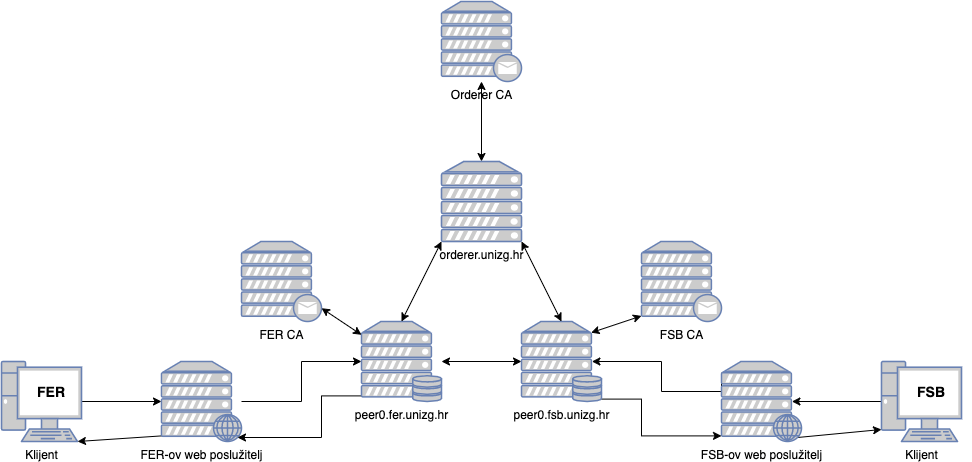
\includegraphics[scale=0.33]{imgs/Arhitektura.png}
\caption{Arhitektura rješenja}
\label{fig:arhitektura}
\end{figure}

Mreža se sastoji od sveukupno tri organizacije. FER, FSB i ordering organizacija. FER i FSB imaju svaka po jedan glavni čvor koji je zadužen za održavanje raspodijeljene glavne knjige, blockchaina i pametnih ugovora. Taj čvor se naziva peer.  Ti peer-ovi, skupa s orderer čvorom, povezani su u jednom kanalu.  Uz peer-ove ključni su i poslužitelji autoriteta za izdavanje certifikata.

\section{Servis članstva}
Autoriteti za izdavanje certifikata izdaju identitete generiranjem javnog i privatnog ključa koji oblikuje par ključeva koji se može koristiti za dokazivanje identiteta. Budući da se privatni ključ nikada ne može javno dijeliti, potreban je mehanizam kako bi se omogućilo dokazivanje identiteta,  i tu dolazi "servis članstva" (eng. Membership Service Provider, skr. MSP). Na primjer, peer koristi svoj privatni ključ za digitalno potpisivanje, ili odobravanje,  transakcije. MSP na ordering usluzi sadrži javni ključ peer-a koji se tada koristi za provjeru da je potpis transakcije validan. Privatni ključ se koristi za proizvodnju potpisa na transakciji koju samo odgovarajući javni ključ, koji je dio MSP-a,  može otključati.  Dakle, MSP je mehanizam koji omogućuje da se identitetu može vjerovati i prepoznati od strane ostatka mreže bez otkrivanja privatnog ključa člana.

Implementacija MSP-a je skup direktorija koje se dodaju konfiguraciji mreže i koristi se za definiranje organizacije iznutra (organizacije odlučuju tko su njeni administratori) i izvana (dopuštajući drugim organizacijama da potvrde da subjekti imaju ovlasti za činjenje onoga što pokušavaju učiniti). Autoriteti za izdavanje certifikata generiraju potvrde koje predstavljaju identitete,  MSP sadrži popis odobrenih identiteta.

MSP se pojavljuje u dvije domene:
\begin{itemize}
\item Lokalna - definirani su za klijente i čvorove (peer i orderer). Svaki čvor mora imati lokalni MSP.
\item Kanalska - definiraju administrativna prava i prava sudjelovanja na razini kanala.  Identificira tko ima vlasti na razini kanala.  Svaka organizacija koja sudjeluje u kanalu mora imati MSP definiran za to.  MSP sustava uključuje MSP svih organizacija koje sudjeluju u ordering servise.  Lokalni MSP-ovi su definirani samo na datotečnom sustavu čvora ili korisnika.  Kanalni MSP je također instanciran na datotečnom sustavu svakog čvora u kanalu i čuva se sinkroniziranim konsenzusnim protokolom.
\end{itemize}

Organizacija se također može podijeliti u više organizacijskih jedinica (eng. Organizational Unit, skr. OU), od kojih svaka ima određeni skup odgovornosti, koje se nazivaju i afilijacije.   Navođenje OU-a nije obavezno. Ako se OU ne koriste, svi identiteti koji su dio MSP-a - kako su identificirani u korijenskim i posredničkim CA direktorijima - smatrat će se članovima organizacije.

Uz to, postoji posebna vrsta OU, koja se ponekad naziva OU čvora, a koja se može koristiti za dodjeljivanje uloge identitetu. Ove uloge OU čvora definirane su u datoteci "/msp/config.yaml" i sadrže popis organizacijskih jedinica čiji se članovi smatraju dijelom organizacije koju predstavlja ovaj MSP. To je osobito korisno kada želite ograničiti članove organizacije na one koji imaju identitet (potpisan od jednog od MSP-a određenih CA-a) s određenom ulogom OU čvora. 

Da bi se koristile uloge OU čvora, mora biti omogućena značajka "klasifikacija identiteta" za mrežu. Kada se koristi struktura MSP-a koja se temelji na mapi, to se postiže omogućavanjem "Node OU" u datoteci config.yaml koja se nalazi u korijenu mape MSP:

\begin{verbatim}
NodeOUs:
  Enable: true
  ClientOUIdentifier:
    Certificate: cacerts/localhost-7054-ca-fer.pem
    OrganizationalUnitIdentifier: client
  PeerOUIdentifier:
    Certificate: cacerts/localhost-7054-ca-fer.pem
    OrganizationalUnitIdentifier: peer
  AdminOUIdentifier:
    Certificate: cacerts/localhost-7054-ca-fer.pem
    OrganizationalUnitIdentifier: admin
  OrdererOUIdentifier:
    Certificate: cacerts/localhost-7054-ca-fer.pem
    OrganizationalUnitIdentifier: orderer
\end{verbatim}

U ovom primjeru nalaze se 4 moguće uloge:
\begin{itemize}
\item klijent (eng.  \textit{client})
\item peer
\item administrator (eng.  \textit{admin})
\item poravnavatelj (eng.  \textit{orderer})
\end{itemize}

\begin{figure}[htb]
\centering
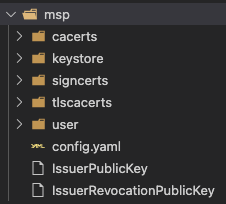
\includegraphics{imgs/msp-folder.png}
\caption{Struktura msp direktorija}
\label{fig:msp}
\end{figure}

Struktura MSP direktorija prikazana na slici \ref{fig:msp}:

\begin{itemize}
\item \textit{config.yaml} - koristi se za konfiguriranje značajke klasifikacije identiteta u Fabricu omogućavanjem "Node OUs" i definiranjem prihvaćenih uloga;
\item \textit{cacerts} - ovaj direktorij sadrži popis samopotpisanih X.509 certifikata korijenskih CA-a kojima vjeruje organizacija koju predstavlja ovaj MSP;
\item \textit{signcerts} - za peer ili orderer (ili u lokalnom MSP-u klijenta) ovaj direktorij sadrži certifikat čvora koji je izdao CA;
\item \textit{keystore} - ovaj direktorij sadrži privatni ključ;
\item \textit{tlscacerts} - ovaj direktorij sadrži popis samopotpisanih X.509 certifikata korijenskia CA-a kojima ova organizacija vjeruje za sigurnu komunikaciju između čvorova pomoću TLS-a.
\item itd.
\end{itemize}

\section{Peer}
Blockchain mreža se sastoji uglavnom od skupa peer-ova. Peer-ovi su temeljni element mreže jer su poslužitelji glavnih knjiga i pametnih ugovora. Podsjetimo da glavna knjiga nepromjenjivo bilježi sve transakcije generirane pametnim ugovorima (koji su u Fabric-u sadržani u chaincode-u). Pametni ugovori i glavne knjige koriste se za enkapsuliranje zajedničkih procesa i zajedničkih informacija u mreži.
Peer poslužuje instance glavnih knjiga i instance chaincode-ova.
Budući da je peer poslužitelj za glavne knjige i chaincode-ove,  aplikacije i administratori moraju komunicirati s peer-om ako žele pristupiti tim resursima. Zato se peer-ovi smatraju temljnim građevnim blokovima Fabric mreže. 

U ovoj implementaciji koristim 2 peer-a. Jedan FER-ov peer0.fer.unizg.hr i FSB-ov peer0.fsb.unizg.hr. Ova nula poslije peer znači broj peer-a, a u ovom primjeru imamo samo jednog peer-a po organizaciji.  

Transakcija ažuriranja prilično se razlikuje od transakcije upita jer pojedinačni peer ne može samostalno ažurirati glavnu knjigu - za ažuriranje je potreban pristanak ostalih peer-ova u mreži. Peer zahtijeva od ostalih peer-ova u mreži da odobre ažuriranje knjige prije nego što se može primijeniti na lokalnu glavnu knjigu peer-a. Taj se postupak naziva konsenzusom,  koji traje puno dulje od jednostavnog upita. Ali kada svi peer-ovi odobre transakciju,  peer-ovi će obavijestiti svoje povezane aplikacije da je glavna knjiga ažurirana.  Točnije, aplikacije koje žele ažurirati glavnu knjigu uključene su u 3-fazni postupak, koji osigurava da svi peer-ovi u blockchain mreži održavaju svoje glavne knjige međusobno dosljednima.

\begin{itemize}
\item U prvoj fazi aplikacije rade s podskupom odobravajućih peer-ova, od kojih svaki šalje odobrenje predloženog ažuriranja glavne knjige aplikaciji, ali ne primjenjuje predloženo ažuriranje na svoju kopiju glavne knjige.
\item U drugoj fazi,  ova odobrenja prikupljaju se zajedno kao transakcije i pakiraju u blokove.
\end{itemize}

Prva faza - prijedlog.  Faza 1 tijeka transakcije uključuje interakciju između aplikacije i skupa peer-ova - ne uključuje orderer-a. Faza 1 odnosi se samo na aplikaciju koja traži da odobravajući peer-ovi organizacija pristanu na rezultate predloženog pozivanja chaincode-a. Da bi započeli fazu 1, aplikacije generiraju prijedlog transakcije koji šalju svakom od potrebnih skupova peer-ova na odobrenje. Zatim, svaki od ovih odobravajućih peer-ova samostalno izvršava chaincode koristeći prijedlog transakcije za generiranje odgovora na prijedlog transakcije. Ne primjenjuje ovo ažuriranje na glavnu knjigu, već ga jednostavno potpisuje i vraća aplikaciji. Nakon što aplikacija dobije dovoljan broj potpisanih odgovora na prijedlog, prva faza tijeka transakcije je završena.

Faza 2 - redanje i pakiranje transakcija u blokove. Orderer je ključan za ovaj dio procesa, prima transakcije koje sadrže odobrene odgovore na prijedloge transakcija od aplikacija i reda transakcije u blokove.

Faza 3 - validacija i postavljanje.  Posljednja faza tijeka transakcije uključuje distribuciju i provjeru valjanosti blokova od orderer-a do peer-ova, gdje mogu ažurirati glavnu knjigu. Točnije, kod svakog peer-a, svaka transakcija unutar bloka provjerava se kako bi se osiguralo da su je sve relevantne organizacije dosljedno odobrile prije nego što se ažurira glavna knjiga.  Neuspjele transakcije zadržavaju se za reviziju, ali ne mijenjaju glavne knjige.  Faza 3 započinje orderer-om koji distribuira blokove svim peer-ovima povezanim s njim.  Svim peer-ovima povezanim s orderer-om bit će poslana kopija novog bloka. Svaki će peer obrađivati ovaj blok neovisno, ali na potpuno isti način kao i svaki drugi peer na kanalu. Na taj ćemo način vidjeti da se glavna knjiga može održavati dosljednom. Također je vrijedno napomenuti da ne mora svaki peer biti povezan s naručiteljem - vršnjaci mogu kaskadno blokirati druge peer-ove koristeći \textit{gossip} protokol \cite{DBLP:journals/corr/abs-2004-07060},  koji ih također mogu samostalno obraditi.

\section{Glavna knjiga}
U Fabricu, glavna knjiga se sastoji od dva različita, iako povezana, dijela - globalno stanje i blockchain. Svaki od njih predstavlja skup činjenica o skupu poslovnih objekata.

Prvo, postoji globalno stanje - baza podataka koja ima trenutne vrijednosti skupa stanja glavne knjige. Globalno stanje olakšava programu za izravno pristup trenutnoj vrijednosti stanja,  bez da ga mora izračunavati prelaskom kroz dnevnik stanja.  Stanja glavne knjigu su, prema zadanim postavkama izražene kao parovi ključ-vrijednost. Globalno stanje se može često mijenjati, jer se stanja mogu stvoriti, ažurirati i izbrisati.

Drugo, tu je blockchain - dnevnik transakcija koji bilježi sve promjene koje su rezultirale trenutnim globalnim stanjem. Transakcije se prikupljaju unutar blokova koji se dodaju na blockchain - omogućujući pregled povijest promjena koje su rezultirale trenutnim globalnim stanjem. Blockchain struktura podataka je vrlo različita od globalnog stanja, jerjednom napisana, ne može se mijenjati.

Globalno stanje fizički je implementirano kao baza podataka, kako bi se omogućilo jednostavno i učinkovito pohranjivanje i pronalaženje stanja glavne knjige. Stanja glavne knjige mogu imati jednostavne ili složene vrijednosti, a kako bi se to prilagodilo, implementacija baze podataka može se razlikovati,  što omogućuje učinkovitu implementaciju tih vrijednosti. Opcije za bazu podataka globalnog stanja trenutno uključuju LevelDB i CouchDB.

U mom primjeru koristio sam CouchDB.  CouchDB je posebno prikladan izbor kada su stanja glavne knjige strukturirana kao JSON dokumenti jer CouchDB podržava bogate upite i ažuriranje bogatijih tipova podataka koji se često nalaze u poslovnim transakcijama.  Implementacijski,  CouchDB radi u odvojenom procesu operativnog sustava, ali postoji odnos 1:1 između peer-a i instance CouchDB baze podataka. Sve je to nevidljivo za pametni ugovor.

Da ponovimo, Blockchain u Fabricu strukturiran je kao sekvencijalni dnevnik međusobno povezanih blokova, gdje svaki blok sadrži slijed transakcija, a svaka transakcija predstavlja upit ili ažuriranje globalnog stanja.  Blockchain je implementiran kao datoteka. 

\begin{figure}[htb]
\centering
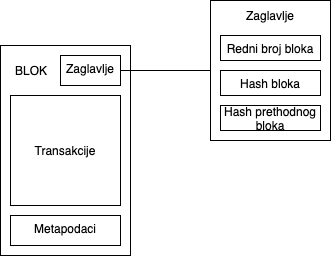
\includegraphics[scale=0.5]{imgs/Block.png}
\caption{Blok}
\label{fig:blok}
\end{figure}

Struktura bloka prikazana na slici \ref{fig:blok}:
\begin{itemize}
\item Zaglavlje - sastoji se od tri polja:
	\begin{itemize}
		\item Redni broj bloka - počinje od 0 (genesis blok) i povećava se za 1 sa svakim dodanim blokom u lanac.
		\item Hash trenutnog bloka - hash svih transakcija koje trenutni blok sadrži.
		\item Hash prethodnog bloka
	\end{itemize}

\item Podaci o transakcijama - ovaj dio sadrži popis transakcija poredanih redom. Zapisuje se kada je blok kreiran od orderer servisa.
\item Metapodaci o bloku - ovaj dio sadrži certifikat i potpis tvorca bloka koji se koristi za provjeru bloka na mrežnim čvorovima.  Postavljač bloka dodaje pokazatelj vrijedi/ne vrijedi za svaku transakciju u "bitmap"-u koja se također nalazi u metapodacima bloka,  kao i hash kumulativnih ažuriranja stanja do i uključujući taj blok,  kako bi se otkrilo račvanje (eng. fork) stanja.  Ovaj dio nije ulaz u funkciju za izračunavanje hash-a bloka.
\end{itemize}

\begin{figure}[htb]
\centering
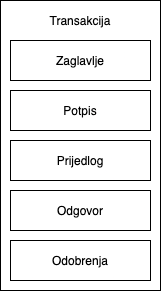
\includegraphics[scale=0.5]{imgs/Transakcija.png}
\caption{Transakcija}
\label{fig:transakcija}
\end{figure}

Struktura transakcije prikazana na slici \ref{fig:transakcija}:
\begin{itemize}
\item \textbf{zaglavlje} - bitni metapodaci o transakciji, na primjer, naziv odgovarajućeg chaincode-a i njegova verzija;
\item \textbf{potpis} - kriptografski potpis,  stvoren od strane klijentske aplikacije. Ovo se polje koristi za provjeru da detalji transakcije nisu kompromitirani, jer za njegovo generiranje potreban je privatni ključ aplikacije;
\item \textbf{prijedlog} - kodira ulazne parametre koje aplikacija šalje pametnom ugovoru koji kreira predloženo ažuriranje glavne knjige. Kada se izvrši pametni ugovor, ovaj prijedlog pruža skup ulaznih parametara koji, u kombinaciji s trenutnim globalnim stanjem, određuju novo globalno stanje;
\item \textbf{odgovor} - bilježi globalno stanje prije i poslije, kao skup za čitanje i upisivanje (eng. Read-Write set, skr. RW-set). To je rezultat pametnog ugovora i ako se transakcija uspješno potvrdi, primijenit će se na glavnu knjigu i ažurirati globalno stanje;
\item \textbf{odobrenja}- ovo je popis potpisanih odgovora na transakcije svake potrebne organizacije dovoljan da zadovolji politiku odobrenja.
\end{itemize}
\section{Poravnavanje transakcija}
Mnogi distribuirani blockchaini, poput Ethereuma i Bitcoina, nemaju ograničen pristup, što znači da bilo koji čvor može sudjelovati u procesu konsenzusa, pri čemu se transakcije poredavaju i grupiraju u blokove. Zbog ove činjenice, ti se sustavi oslanjaju na algoritme vjerojatnog konsenzusa koji na kraju jamče dosljednost glavne knjige do visokog stupnja vjerojatnosti, ali koji su i dalje ranjivi na divergentne glavne knjige (poznati i kao "fork" glavne knjige), gdje različiti sudionici mreže imaju drugačiji pogled na prihvaćeni redoslijed transakcija.

U Hyperledger Fabric-u ima čvor pod nazivom \textit{orderer} koji radi poredavanje transakcija, koji zajedno s drugim čvorovima orderer-a čini uslugu poredavanja.  Budući da se Fabric dizajn oslanja na determinističke konsenzusne algoritme, bilo koji blok potvrđen od strane peer-a zasigurno će biti konačan i točan.  Glavne knjige ne mogu divergirati na način na koji mogu u mnogim drugim distribuiranim blockchain mrežama bez ograničenog pristupa.

Osim promicanja konačnosti,  odvajanje odobrenja izvođenja chaincodea (što se događa na peer-ovima) od poredavanja transakcija daje prednosti Fabric-u u performansama i skalabilnosti i uklanjanje uskih grla koje se mogu pojaviti kada izvršenje i poredavanje provode isti čvorovi.

U svojoj implementaciji odlučio sam orderer čvor staviti u zasebnu orderer organizaciju .  Koristim samo jedan orderer čvor orderer.unzig.hr radi jednostavnije demonstracije Fabric radnog okvira. Za bolje djelovanje Fabric mreže poželjno je imati 3 ili 5 ordering čvora. 


\section{Chaincode}
Chaincode je program napisan u programskom jeziku Go,  Node.js ili Java koji implementira propisano sučelje.  Chaincode radi u zaštićenom Dockerovom kontejneru izoliranom od procesa odobravajućeg peer-a.  Chaincode inicijalizira stanje glavne knjige i upravlja njime putem transakcija koje prima od aplikacija.

Chaincode obično obrađuje poslovnu logiku s kojom su se složili članovi mreže, pa se može smatrati "pametnim ugovorom". Ažuriranja glavne knjige stvorena chaincode-om opsega su isključivo na taj chaincode i ne može im se izravno pristupiti drugim chaincode-om. Međutim, unutar iste mreže, s obzirom na odgovarajuće dopuštenje,  chaincode može pozvati drugi chaincode za pristup svom stanju.

Životni ciklus chaincode-a u Fabric mreži zahtjeva da se ogranizacije slože u parametrima koji definiraju chaincode, kao što su ime, verzija i politiku odobravanja.  Članovi kanala dolaze do sporazuma kroz sljedeća četiri koraka, ali ne moraju sve organizacije napraviti svaki korak:

\begin{enumerate}
\item Pakiranje chaincode-a - ovaj korak može napraviti jedna,  više ili sve organizacije u kanalu.  Naredba koja se koristi za ovaj korak je: 
\textit{peer lifecycle chaincode package}

\item Instaliranje chaincode-a na peer - svaka organizacija koja će koristiti chaincode kako bi odobrila transakciju ili zatražila podatke s glavne knjige mora izvršiti ovaj korak.  Naredba:
\textit{peer lifecycle chaincode install}

\item Odobrenje definicije chaincode-a za organizaciju - svaka organizacija koja će koristiti chaincode mora izvršiti ovaj korak.  Definiciju chaincode-a mora odobriti dovoljan broj organizacija kako bi se zadovoljile politike životnog vijeka kanala (većina,  prema zadanim postavkama) prije nego što se chaincode može pokrenuti na kanalu.  Naredba:
\textit{peer lifecycle chaincode approveformyorg}

\item  Postavljanje definicije chaincode-a na kanal - transakciju postavljanja mora predati jedna organizacija nakon što je potreban broj organizacija na kanalu odobrilo chaincode. Podnositelj zahtjeva prvo prikuplja odobrenja od dovoljnog broja organizacija,  a zatim predaje transakciju kako bi postavio definiciju chaincode-a na kanal. Naredba:
\textit{peer lifecycle chaincode commit}
\end{enumerate}

U ovoj implementaciji koristio sam dva chaincode-a. Chaincode za ERC-20 token koji predstavlja bodove za menzu i chaincode za ERC-721 token koji predstavlja rektorovu nagradu. Pisani su u JavaScript programskom jeziku.

\section{Kanal}

Kanal je primarni komunikacijski mehanizam kojim članovi konzorcija mogu međusobno komunicirati. U mreži mogu biti više kanala. Kanali su korisni jer pružaju mehanizam za privatne komunikacije i privatne podatke između članova konzorcija. Kanali pružaju privatnost od drugih kanala, ali i od mreže. Fabric je moćan u tom pogledu, jer organizacijama omogućuje dijeljenje infrastrukture i čuvaju je privatnom u isto vrijeme. Ovdje nema kontradikcije - različite konzorcije unutar mreže imat će potrebu za različitim informacijama i procesima da se na odgovarajući način dijele, a kanali pružaju učinkovit mehanizam za to. Kanali pružaju učinkovito dijeljenje infrastrukture uz zadržavanje privatnosti podataka i komunikacije.

\section{Klijent}

Klijentska aplikacija se sastoji od dva dijela,"prednji" (eng. \textit{frontend}) - sučelje i "stražnji" (eng. \textit{backend}) - poslužitelj. Ovakva struktura je standardna u aplikacijama koje koriste Hyperledger Fabric mrežu.  Omogućava odvajanje direktne komunikacije između aplikacije i mreže te aplikacije i klijenta. Prednost tome je jednostavnije korištenje i programiranje aplikacije. 
%O KLIJENTSKOJ APLIKACIJI
\subsection{Sučelje}

"Prednji" dio aplikacije ili popularno nazvano \textit{frontend},  programirano je koristeći radni okvir Angular.  Angular je radni okvir otvorenog koda i napisan je u programskom jeziku TypeScript od strane Angular tima u Google-u. Ovaj radni okvir,  koji se koristi za izradu web aplikacija, uz korištenje Angular Material biblioteke čini programiranje sučelja relativno jednostavnim. 

% ANGULAR
\subsection{Backend}

"Stražnji" dio aplikacije ili \textit{Backend}, programirao sam koristeći TypeScript programski jezik i Node.js \textit{runtime} okruženje.  Ovaj dio aplikacije izveden je uz REST načela \cite{BATTLE200861} programiranja web poslužitelja. Uz Node.js koristio sam i radni okvir Express.js koji olakšava i poboljšava programiranje aplikacija na poslužiteljskoj strani.%citat rest

U "običnim" web aplikacijama, ovaj dio bi komunicirao s "običnom" bazom podataka, na primjer MySQL, PostgreSQL i slično. U ovom primjeru komunicira s Fabric blockchain mrežom, koja zapravo služi kao baza podataka, raspodijeljena baza podataka do koje pristup imaju, i svi podaci su jednaki, sve organizacije koje su članovi te mreže ili kanala unutar te mreže. 

Tijek aplikacije na primjeru stvaranja bodova za menzu:

\begin{enumerate}
\item klijent otvori aplikaciju u svom internetskom poslužitelju te napravi zahtjev za stvaranje novih bodova za menzu;
\item taj zahtjev preko HTTP protokola stiže na Node.js poslužitelj;
\item poslužitelj obradi zahtjev i ako je zahtjev u redu, šalje zahtjev dalje prema blockchain mreži, točnije poziva metodu "Mint" erc20 chaincode-a;
\item chaincode obrađuje zahtjev i provjerava identitet pošiljatelja. Ako je sve u redu, stvara nove bodove i dodaje ih u ukupan zbroj bodova u mreži i dodaje ih na račun stvaratelja;
\item nakon što server primi poruku od mreže da su bodovi uspješno stvoreni, vraća odgovor klijentu koji na svom ekranu vidi nove bodove.
\end{enumerate}


\chapter{Zaključak}
Blockchain je tehnologija koja sasvim sigurno ostavlja veliki utjecaj u četvrtoj industrijskoj revoluciji. Predstavlja novi način na koji razmišljamo o djeljenju podataka. Donosi rješenja za probleme koje se dugo vremena nije moglo riješiti. To je naročito zainteresiralo poslovni svijet.  Stoga su nastale razne implementacije te tehnologije koje se natječu u rješavanju poslovnih problema, a u ovom radu smo spomenuli Quorum, Corda i Hyperledger Fabric. 

Hyperledger Fabric je radni okvir za implementaciju blockchaina s ograničenim pravom pristupa koji je korišten za implementacijski dio rada. Fabric je najmodularniji i pokazuje najbolje performanse od svih prethodno spomenutih izvedbi blockchaina s ograničenim pravom pristupa.

Na jednostavnom primjeru bodova u menzi i rekotorovih nagrada između FER-a i FSB-a pokazalo se i analiziralo kako izgleda konkretan primjer korištenja Hyperledger Fabric platforme. Sama blockchain mreža se koristi kao raspodijeljena baza podataka koja se dijeli između FER-a i FSB-a, a klijentska aplikacija je inicijator transakcija kojima se dolazi do podataka na mreži ili ih se ažurira. 

\bibliographystyle{fer}
\bibliography{literatura}


\begin{sazetak}
Sažetak na hrvatskom jeziku.

\kljucnerijeci{ključne riječi, odvojene zarezima.}
\end{sazetak}

% TODO: Navedite naslov na engleskom jeziku.
\engtitle{Permissioned blockchain and distributed ledger technologies with smart contracts}
\begin{abstract}
Abstract.

\keywords{Keywords.}
\end{abstract}

\end{document}
